\section{Overview: High-level components and their interaction}
\label{s:overview}%
Inside the CKB application we are describing in this document we can distinguish five high-level components: the \textbf{CKB server}, the \textbf{Evaluator Server}, the \textbf{DBMS}, the \textbf{Mail Server}, and the \textbf{WebAppUI}.
The \textbf{CKB server} is the main component of our system and contains every piece of business logic required to satisfy the goals we specified in the RASD.
The \textbf{Evaluator server} has the purpose to run some analysis on the code written by a team participating in battles, and to compute a score using the results of such analysis.
Since these two servers need to interact with each other they expose some APIs to do just so. 
The role of the \textbf{DBMS} is the usual one, interacting with a database by executing some operations on it (further information about the database is in the \textit{Other Design Decisions section} [\ref{ss:other-design-decisions-database}]).
The \textbf{Mail Server} is used to send notifications by e-mail to the platform’s users. At last, the \textbf{WebAppUI} represents the web application from the client's perspective.
\pagebreak
\section{Component view}
\label{s:component-view}%
\subsection*{Client}
\begin{itemize}
  \item \textbf{WebAppUI}: represents the web application, which is reachable by any browser and usable only after a user has been authenticated using the \textbf{\textit{AuthInterface}}. It allows both STs and EDs to perform a certain set of actions based on the type of user by using the \textbf{\textit{DashboardInterface}}
\end{itemize}
\subsection*{Server}
\begin{itemize}
  \item \textbf{AuthenticationService}: provides the set of procedures required to handle the authentication of a user into the system (i.e., login, registration)
  \item \textbf{DashboardManager}: used as an intermediary between the \textit{WebAppUI} and the other components of the server to provide the web application only the functionality strictly necessary for it to work properly.
  \item \textbf{CompetitionManager}: handler of all functionalities regarding competitions (for both STs and EDs) excluding badges, which management has been delegated to the \textit{BadgeMonitor} component
  \item \textbf{Battle Manager}: same as the \textit{CompetitionManager} but transposed to handle battles. Delegates the team creation/deletion to the \textit{TeamManager}
  \item \textbf{TeamManager}: used to manage the teams used by the STs to participate to battles, it also includes the invite handling
  \item \textbf{BadgeManager}: its purpose is to deal with badges, create/remove a badge with its related rule, and perform checks to verify if a ST enrolled in a competition satisfies any badge rule defined in such competition
  \item \textbf{NotificationService}: its main goal is to implement procedures to send various types of notifications to the application's users; to send such notifications (mails) it uses the \textbf{\textit{MailAPI}} provided by the \textit{MailServer}
  \item \textbf{DataManager}: mediator between the model components and the \textit{DBMS}; it uses the procedures provided by the \textbf{\textit{DBMS\_API}} to implement a set of functions, which have the sole purpose of manipulating the database or retrieving information from it
  \item \textbf{EvaluatorController}: it is called through the \textbf{\textit{EvaluationAPI}} by \textit{GitHub Actions} on each commit performed by a team. Its purpose is to control the evaluation process by calling the \textit{StaticAnalyzer} and the \textit{CodeEvaluator} to perform the proper checks on the last committed code. Moreover, it uses the functions provided by the \textbf{\textit{EvaluatorInterface}}, \textbf{\textit{AnalyzerInterface}}, \textbf{\textit{ScoreInterface}} to change the configuration of the code evaluator and the static analyzer, with the last interface it sets the score functions used by the \textit{PointManager}
  \item \textbf{CodeEvaluator}: used to execute the source code of a team's repository with the set of test cases provided by the EDs of the current battle. It exposes the \textbf{\textit{EvaluatorInterface}} to be used to configure the evaluator for instance in terms of test cases or maximum execution time
  \item \textbf{StaticAnalyzer}: provides the \textbf{\textit{AnalyzerInterface}} to configure the static analyzer, which will be used to analyze some input code. Such analysis will return some results, which can be sent to the \textit{PointManager} through the proper interface still provided by the PointManager (this holds also for the \textit{CodeEvaluator})
  \item \textbf{PointManager}: as the name suggests, it manages the points assignment. In particular it provides two interfaces that are used by the \textit{StaticAnalyzer} and the \textit{CodeEvaluator} to send the results of their analysis. Such results are put in a score function designed by the EDs to compute the partial score of a single analysis; once the \textit{PointManager} computes the score of both the evaluations (static analysis and code evaluation) it updates the final score of the team in the database

\end{itemize}

\begin{figure}[H]
    \label{fig:component-view}
    \centering
    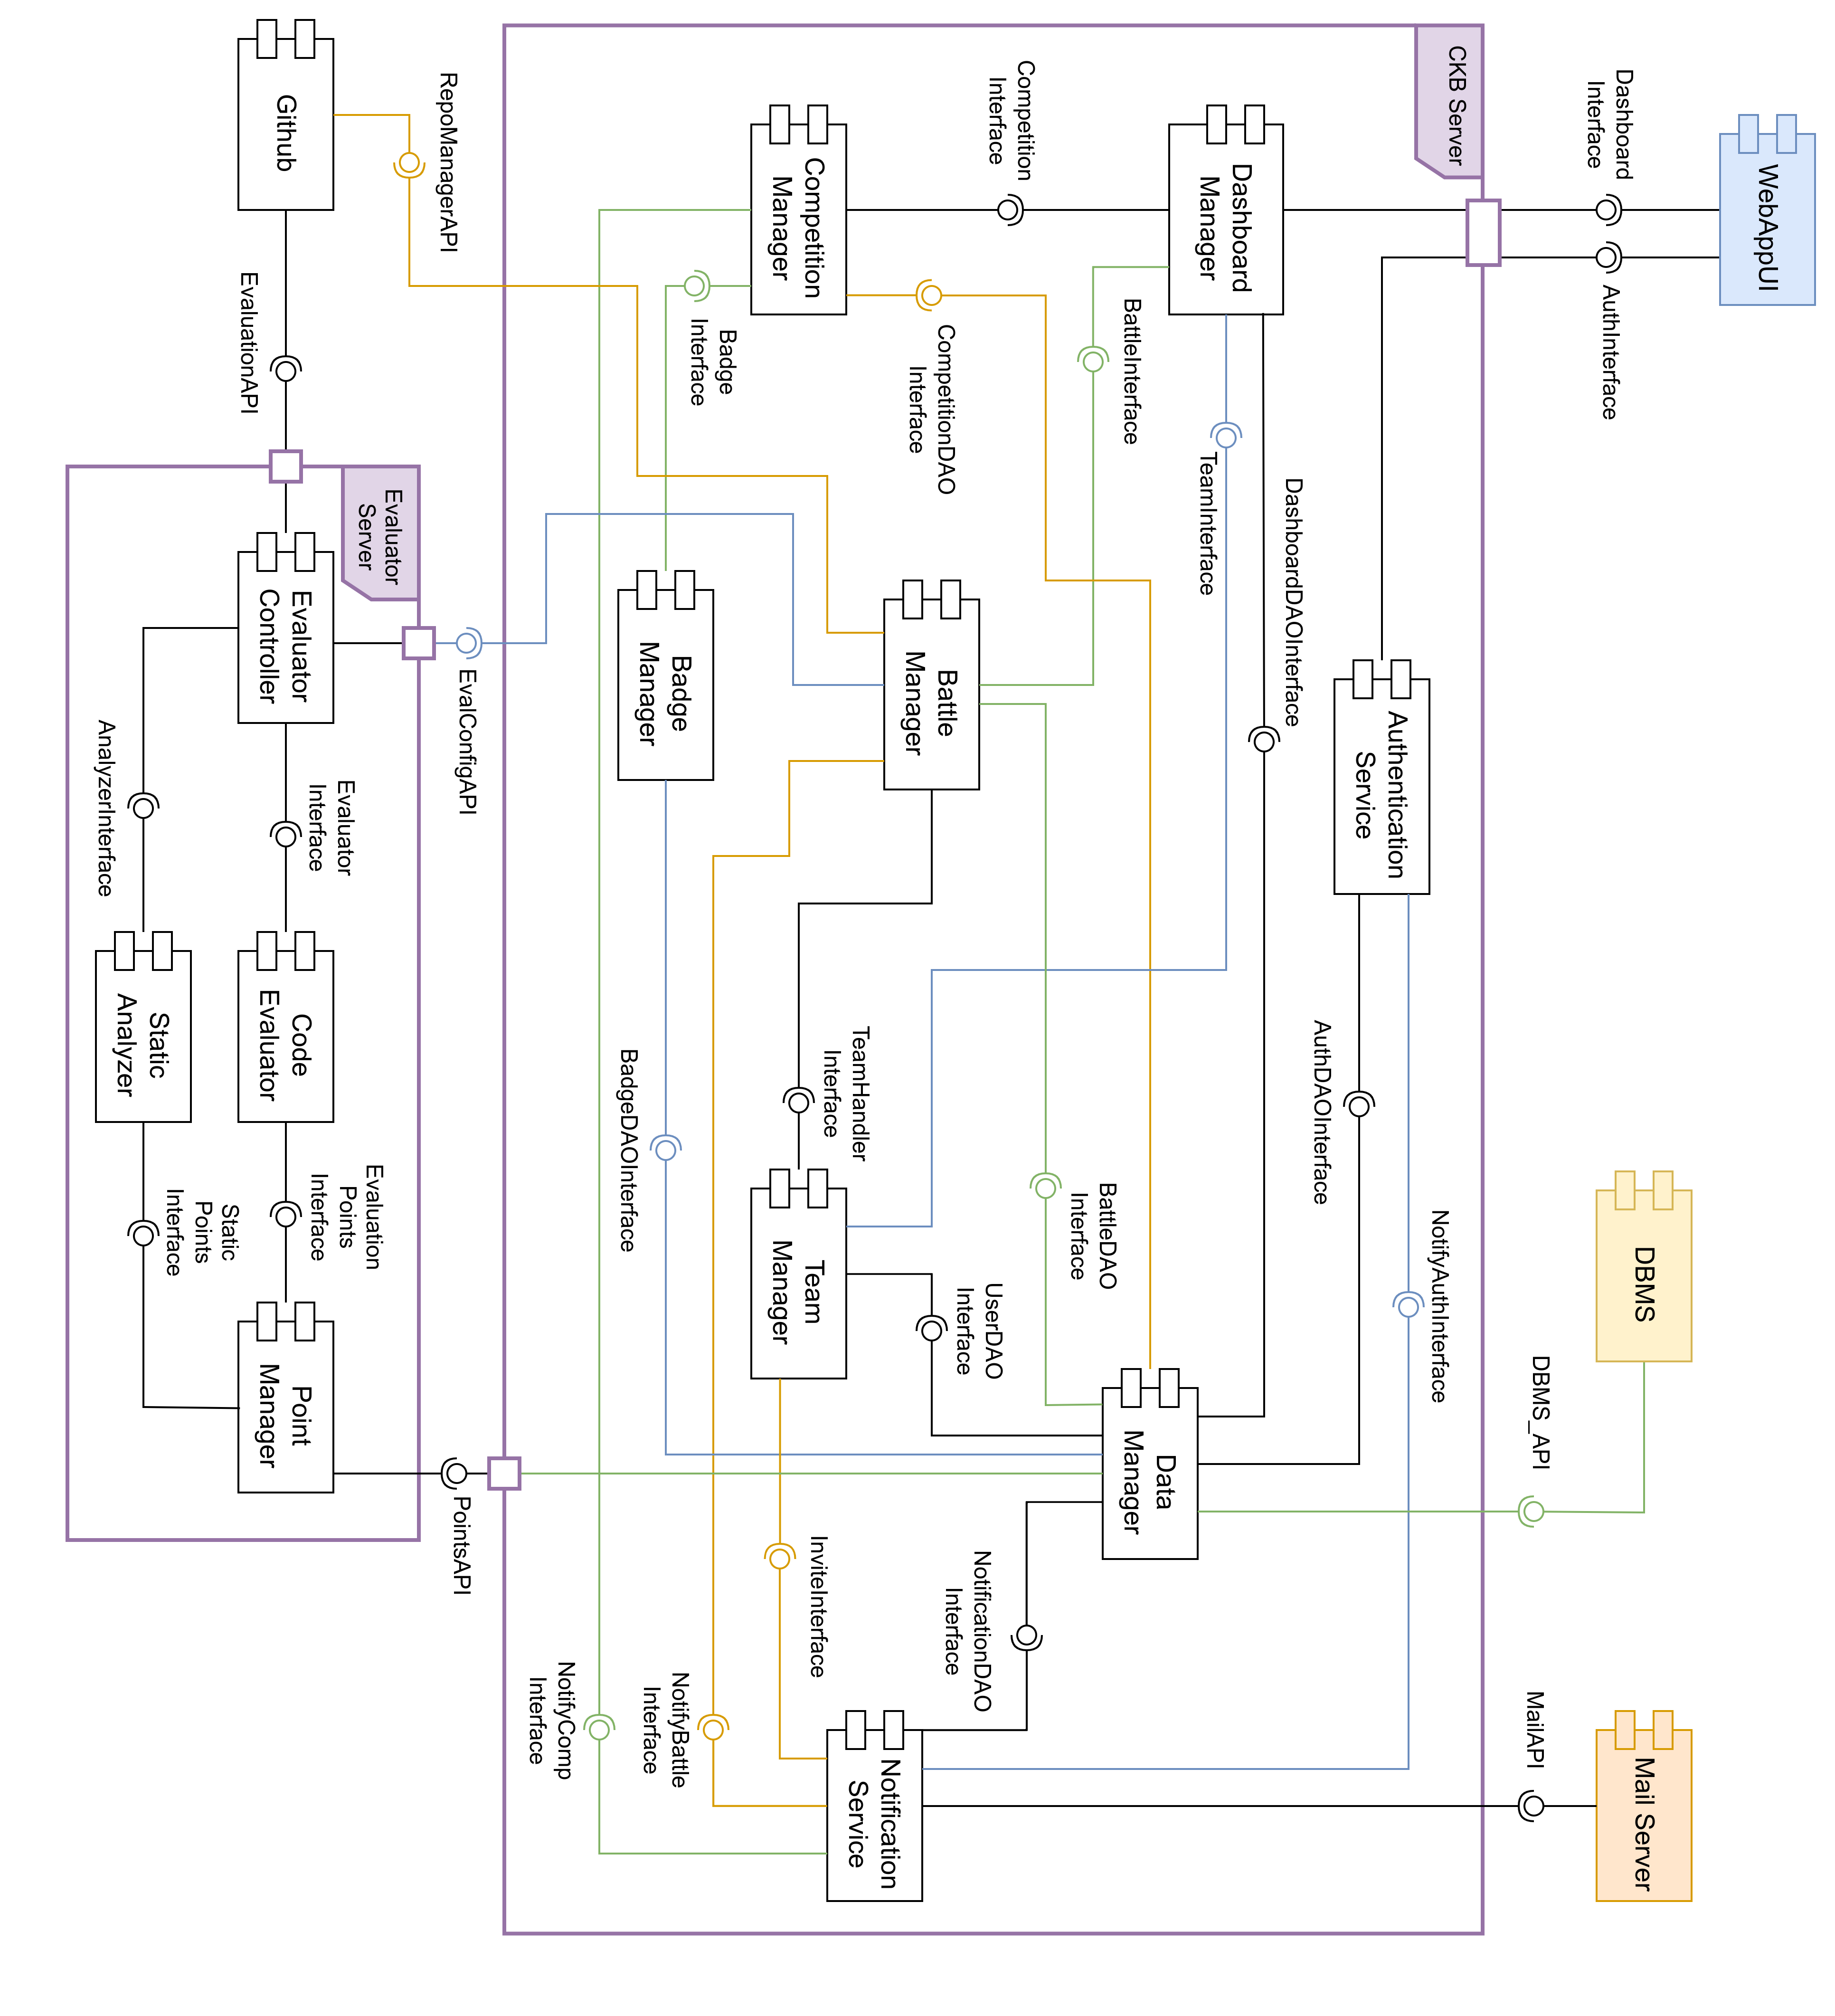
\includegraphics[width=\textwidth, keepaspectratio]{ArchitecturalDesign/componentView.png}
    \caption{Deployment view}
\end{figure}
\newpage

\section{Deployment view}
\label{s:deployment-view}%

The following diagram shows the deployment view of the system. It illustrates the distribution of the components of the system on the different nodes and how they communicate bewteen them. The system is composed by four tiers: the client tier, the application tier, the data tier and the evaluation tier. The client tier is composed by the web browser, which is used by the users to access the application. The application tier is composed by the application servers, which are used to handle the requests from the users and to communicate with the database and with the evaluation servers. The data tier is composed by the database, which is used to store the data of the application. The evaluation tier is composed by the evaluation servers, which include both the static analyzer and the code evaluator.

\begin{figure}[H]
    \label{fig:deployment-view}
    \centering
    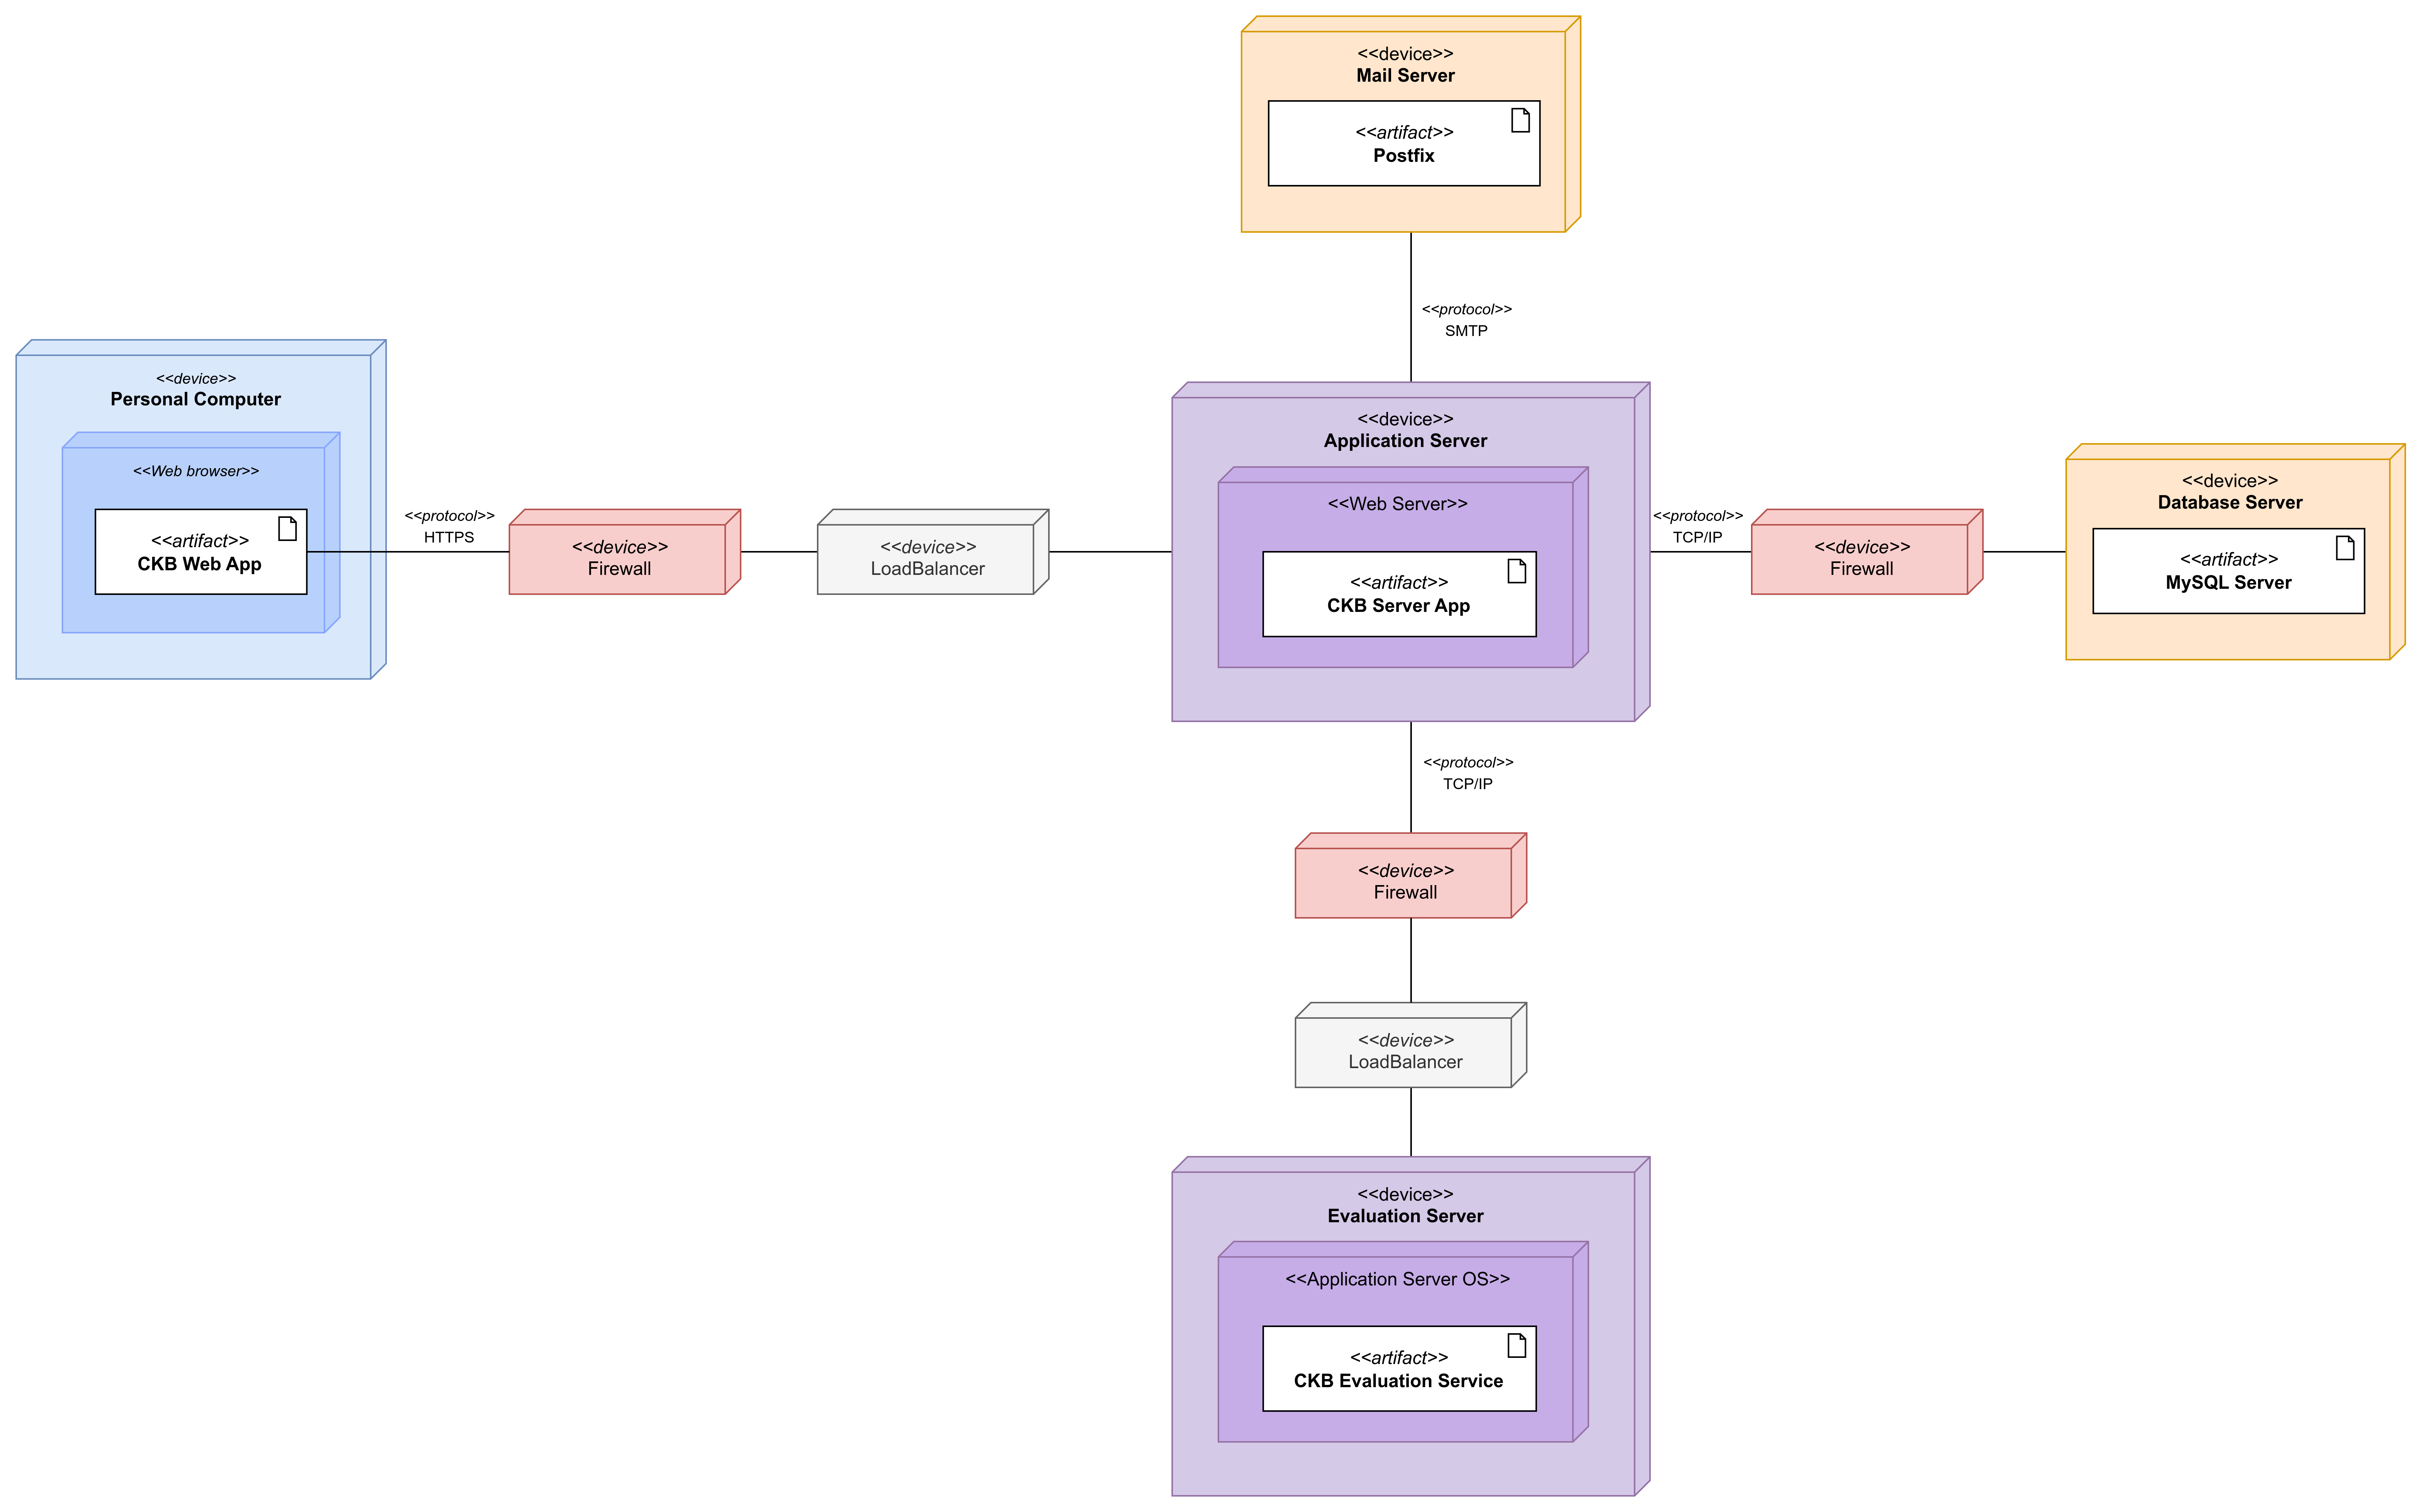
\includegraphics[width=\textwidth]{ArchitecturalDesign/deploymentView.png}
    \caption{Deployment view}
\end{figure}


\subsection{Load Balancing}
Since the CKB will be potentially have a lot of concurrent users, we decided to use a load balancer to distribute the load among multiple servers. This allows us to have a more scalable application, because we can add more servers to the system to handle the increasing load.

A load balacing is also applied for the Evaluation Servers to handle the queue of the new commits to evaluate.

\subsection{Firewall}
To protect the application from external attacks, we decided to use multiple firewall to filter the traffic. In particular, we have a firewall between the client and the load balancer, a firewall between the application servers and the load balancer before the Evaluation Server and a firewall between the application servers and the database. This allows us to have a more secure application, because the firewall will filter the traffic before it reaches the different components of the system.


\section{Runtime view}
\label{s:runtime-view}%
This section contains the sequence diagrams of the most important operations of the system. The diagrams include the component that we have already described in the previous section and the external components that are involved in the operations.

\subsubsection*{User Registration}
\label{ss:registration_diagram}%
When a user wants to register to the system, he/she has to fill in the registration form and submit it. The difference between a ST and an ED is in the information passed with \textit{UserInfo} object, where the ED has to insert also the information about the institution he/she works for.

The whole process is mainly handled by the \textit{Authentication Service} component, that interact with the \textit{Data Manager} component to validate the information and insert the new user into the DBMS.

The system will check if the information inserted are valid and if the user is not already registered. This check is done internally from CKB and if the information are valid and the user is not already registered, the system will insert it into the DBMS and sends an email to the user with a link to confirm the registration, using the \textit{Notification Manager} component. The user will click on the link and the \textit{Authentication Service} will confirm the registration.

If the information inserted are not valid, the user is already registered or the confirmation link is expired, the system will send an error message to the user.

\begin{figure}[H]
  \centering
  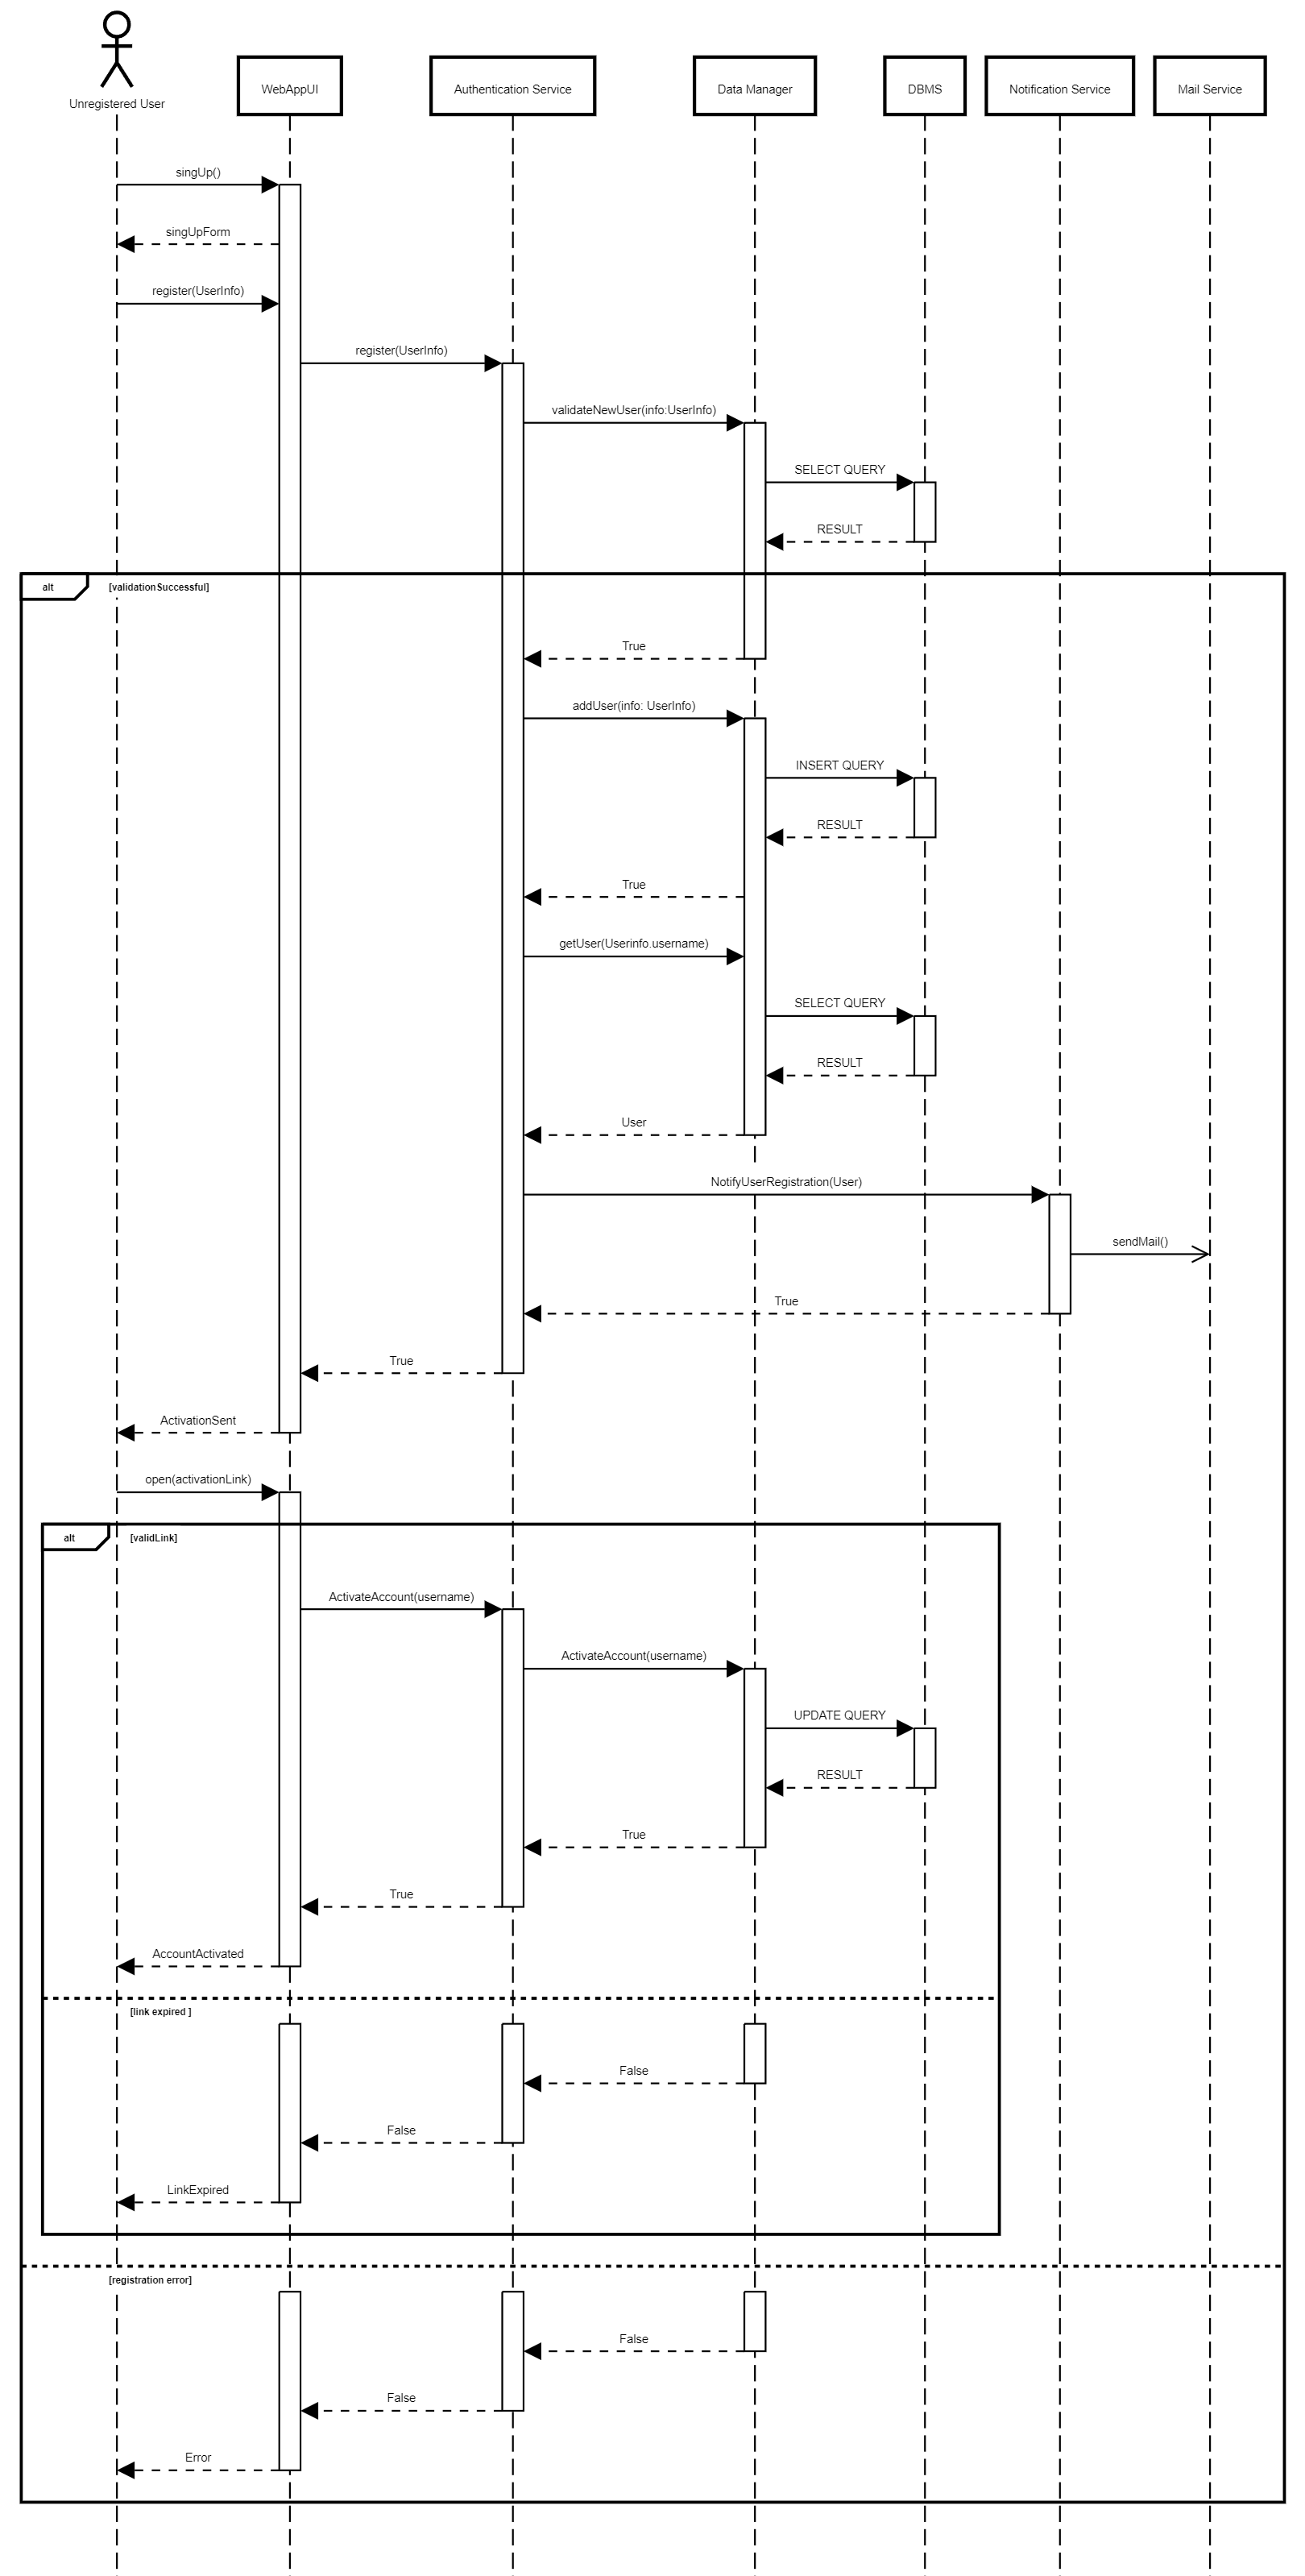
\includegraphics[width=\textwidth,height=\textheight, keepaspectratio]{SequenceDiagrams/01-UserRegistration.png}
  \caption{Registration sequence diagram}
  \label{fig:registratio_diagramn}
\end{figure}

\subsubsection*{User Login}
\label{ss:login_diagram}%
When a user wants to login to the system, he/she has to fill in the login form and submit it. This process is equal for both the ST and the ED. As the User Registration, the whole process is handled by the \textit{Authentication Service} component, that interact with the \textit{Data Manager} component to validate the information. Once the user is logged in, the \textit{Authentication Service} will generate a token for the user, send it to the client and the user can finally access the dashboard.

If the login information are not valid, the system will show an error message to the user.

\begin{figure}[H]
  \centering
  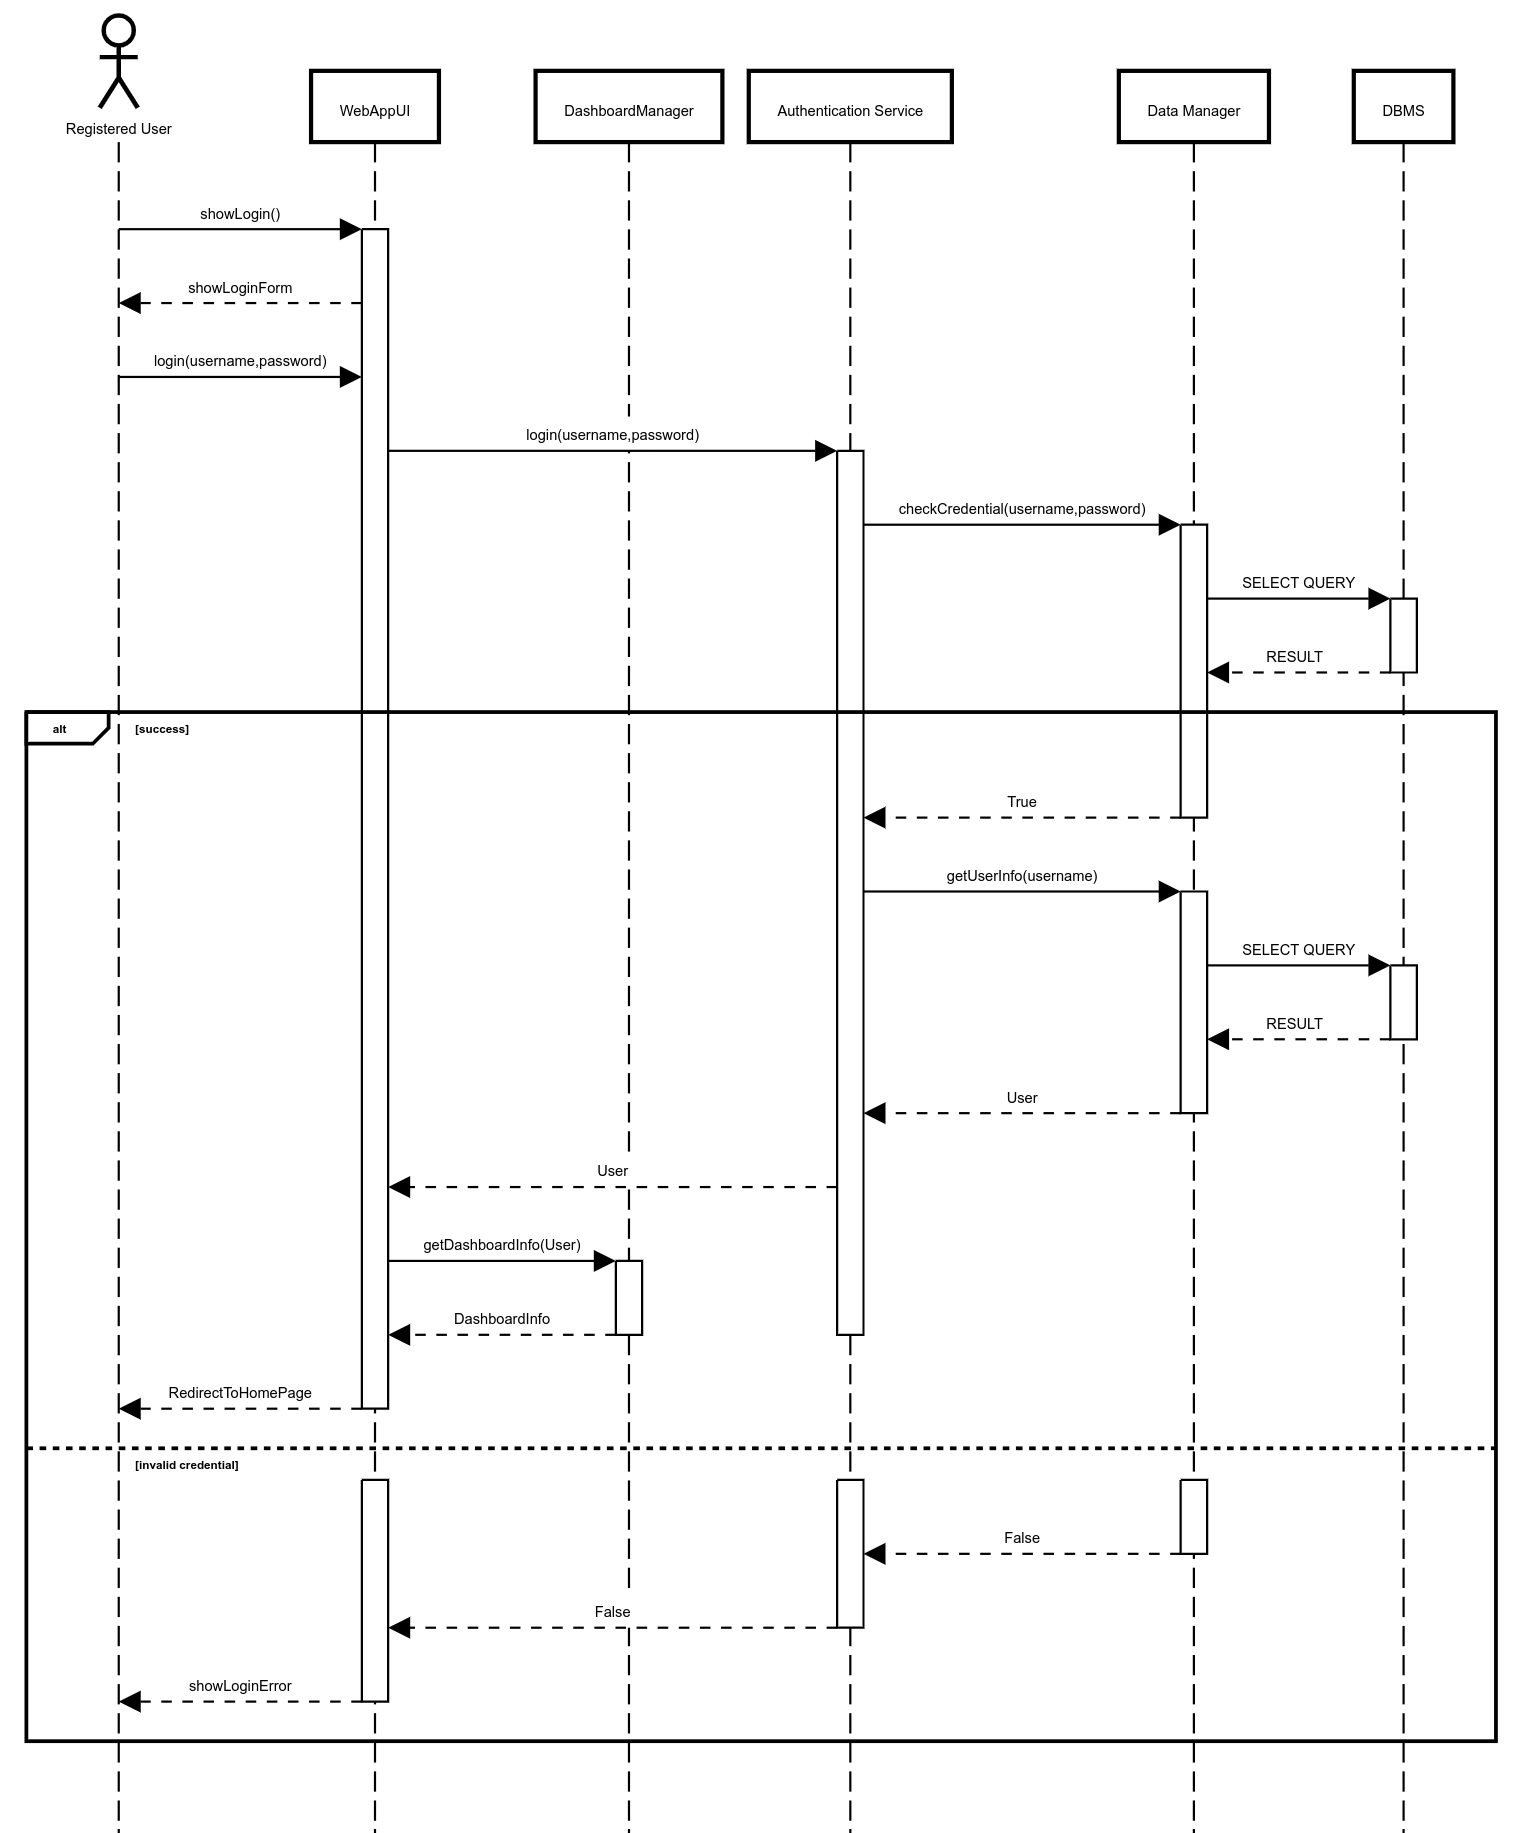
\includegraphics[width=\textwidth,height=0.7\textheight, keepaspectratio]{SequenceDiagrams/02-UserLogin.png}
  \caption{Login sequence diagram}
  \label{fig:login_diagramn}
\end{figure}

\subsubsection*{ED Creates Competition}
\label{ss:create_competition_diagram}
Here is shown how a competition is created by an ED. The ED has to fill in the form with the information about the competition and submit it. The \textit{Competition Manager} component will check if the name is available and if so the competition will be created and inserted into the DBMS using the \textit{Data Manager} component, otherwise a new name will be requested. The system will then returns the competition and will be shown the competition page.

\begin{figure}[H]
  \centering
  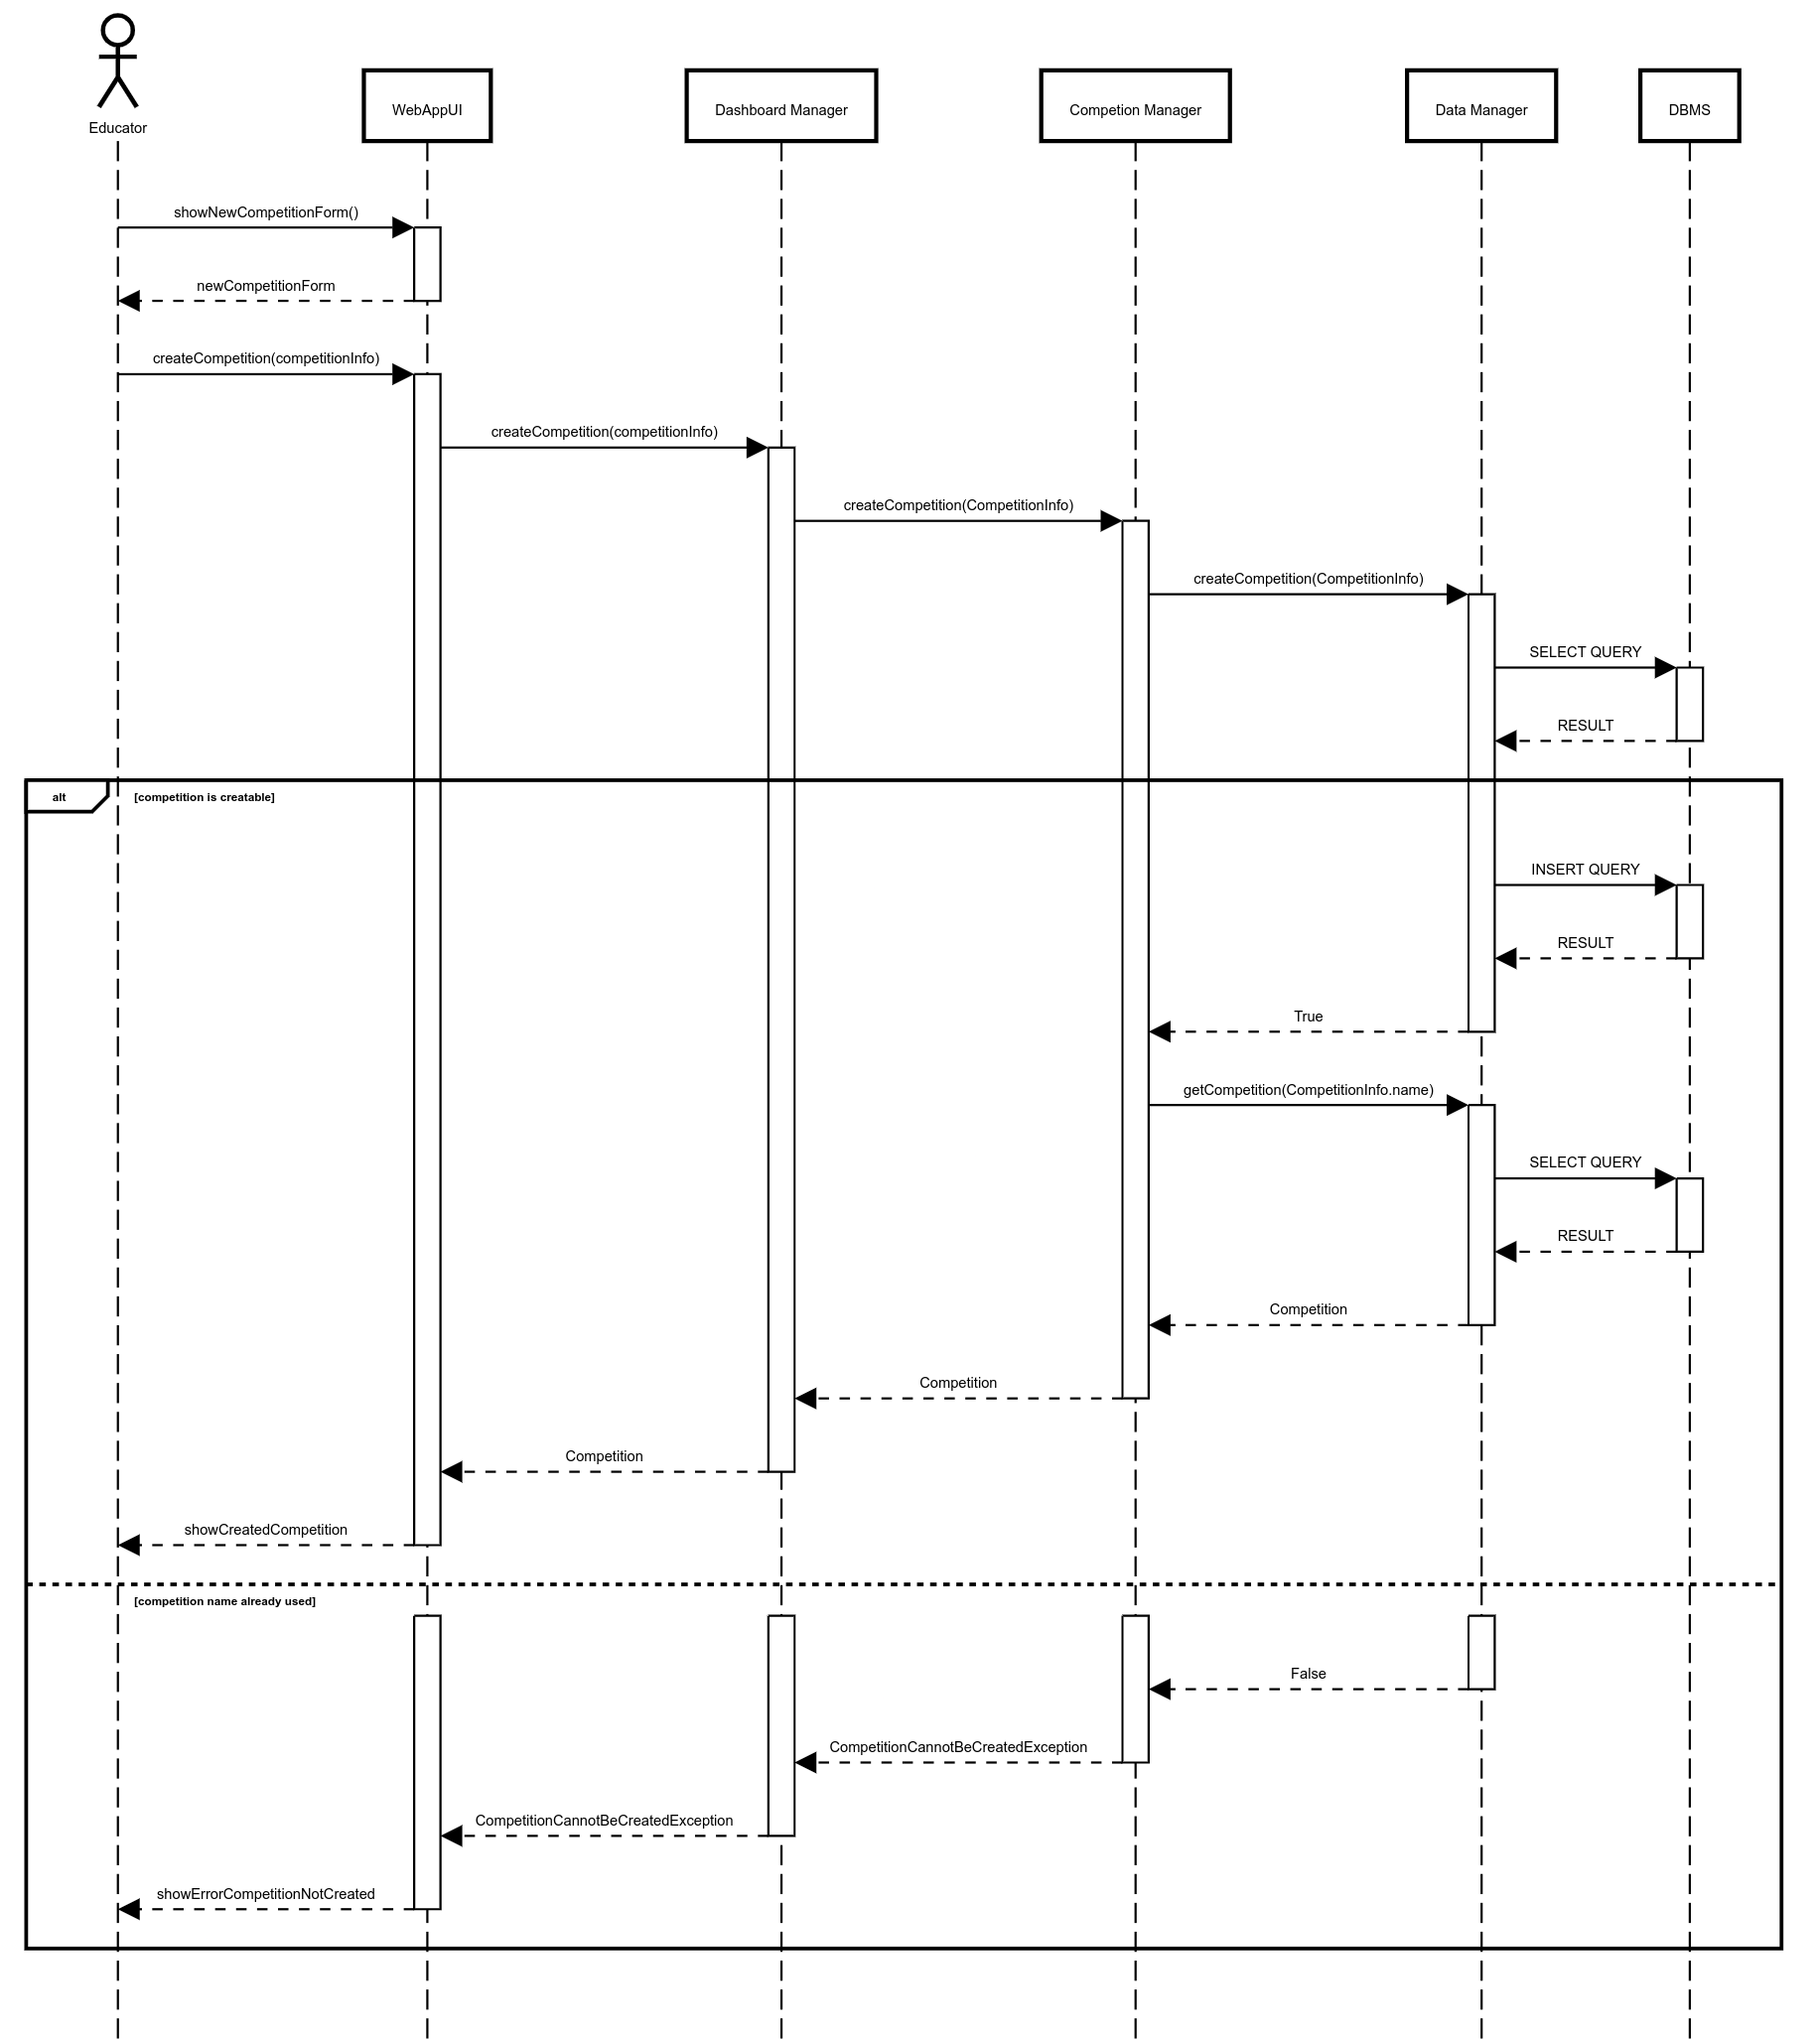
\includegraphics[width=\textwidth,height=0.74\textheight, keepaspectratio]{SequenceDiagrams/04-EducatorCreatesCompetition.png}
  \caption{Create competition sequence diagram}
  \label{fig:create_competition_diagramn}
\end{figure}

\subsubsection*{ST Joins Competition}
\label{ss:join_competition_diagram}
The ST firstly visualize all the available competitions in the platform, then he/she can choose one of them and join it. The \textit{Competition Manager} component will handle both the search of the available competitions and the insertion into the DBMS using the \textit{Data Manager} component. The system will then show a success message to the user.

\begin{figure}[H]
  \centering
  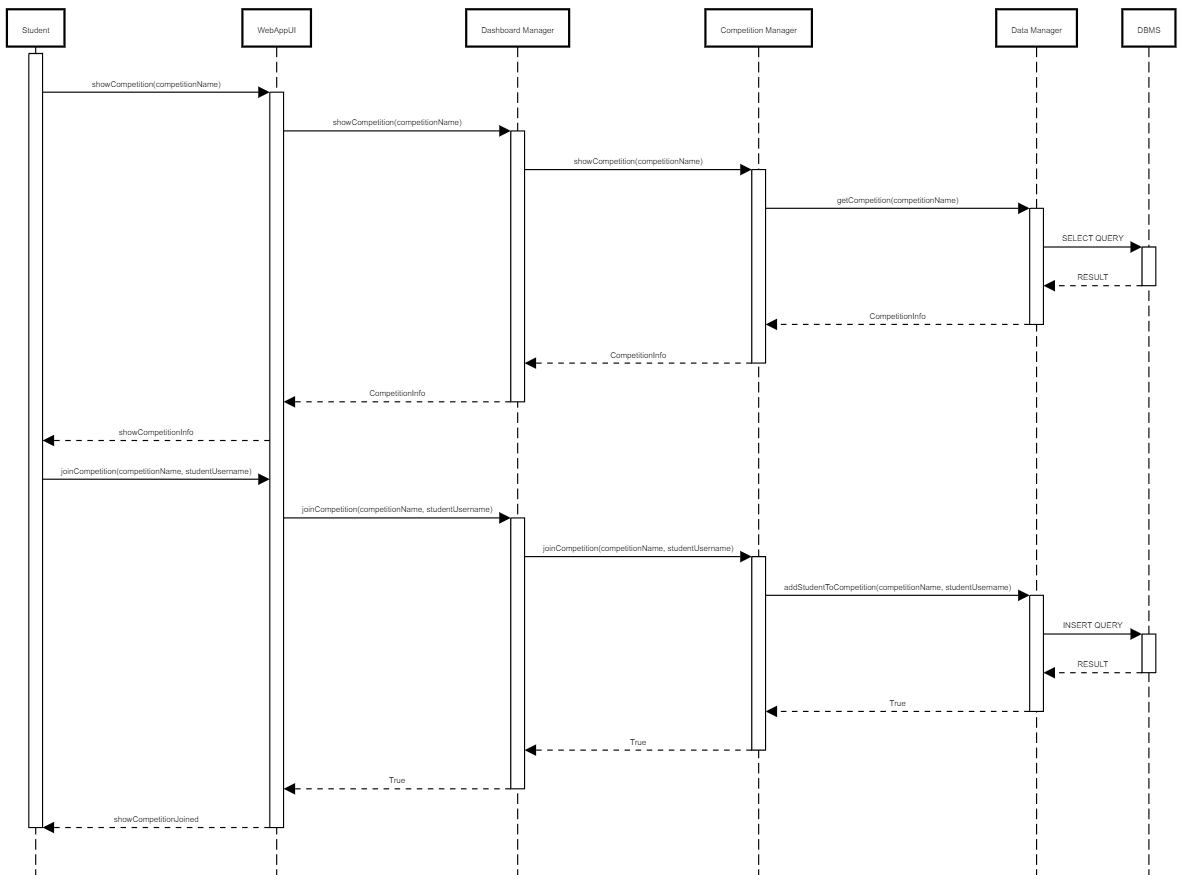
\includegraphics[width=\textwidth,height=\textheight, keepaspectratio]{SequenceDiagrams/05-StudentJoinCompetition.png}
  \caption{Join competition sequence diagram}
  \label{fig:join_competition_diagramn}
\end{figure}

\subsection*{ED Creates Battle}
\label{ss:create_battle_diagram}
When a ED wants to create a battle, he/she needs to be in a competition page that he/she manages. The interaction is divided in two parts: the first one is where the ED inserts the general information about the battle, the name is then validated by the \textit{Battle Manager} component and if it is valid the system will show the second part of the form where the ED can insert the information about the automatic evaluation and static analysis. The \textit{Battle Manager} component will check if the information are valid and if so the battle will be created and inserted into the DBMS using the \textit{Data Manager} component.

If the battle is successfully created, the system will send a notification, through the \textit{Notification Manager} to all the ST enrolled in the competition where the battle has been created.

\begin{figure}[H]
  \centering
  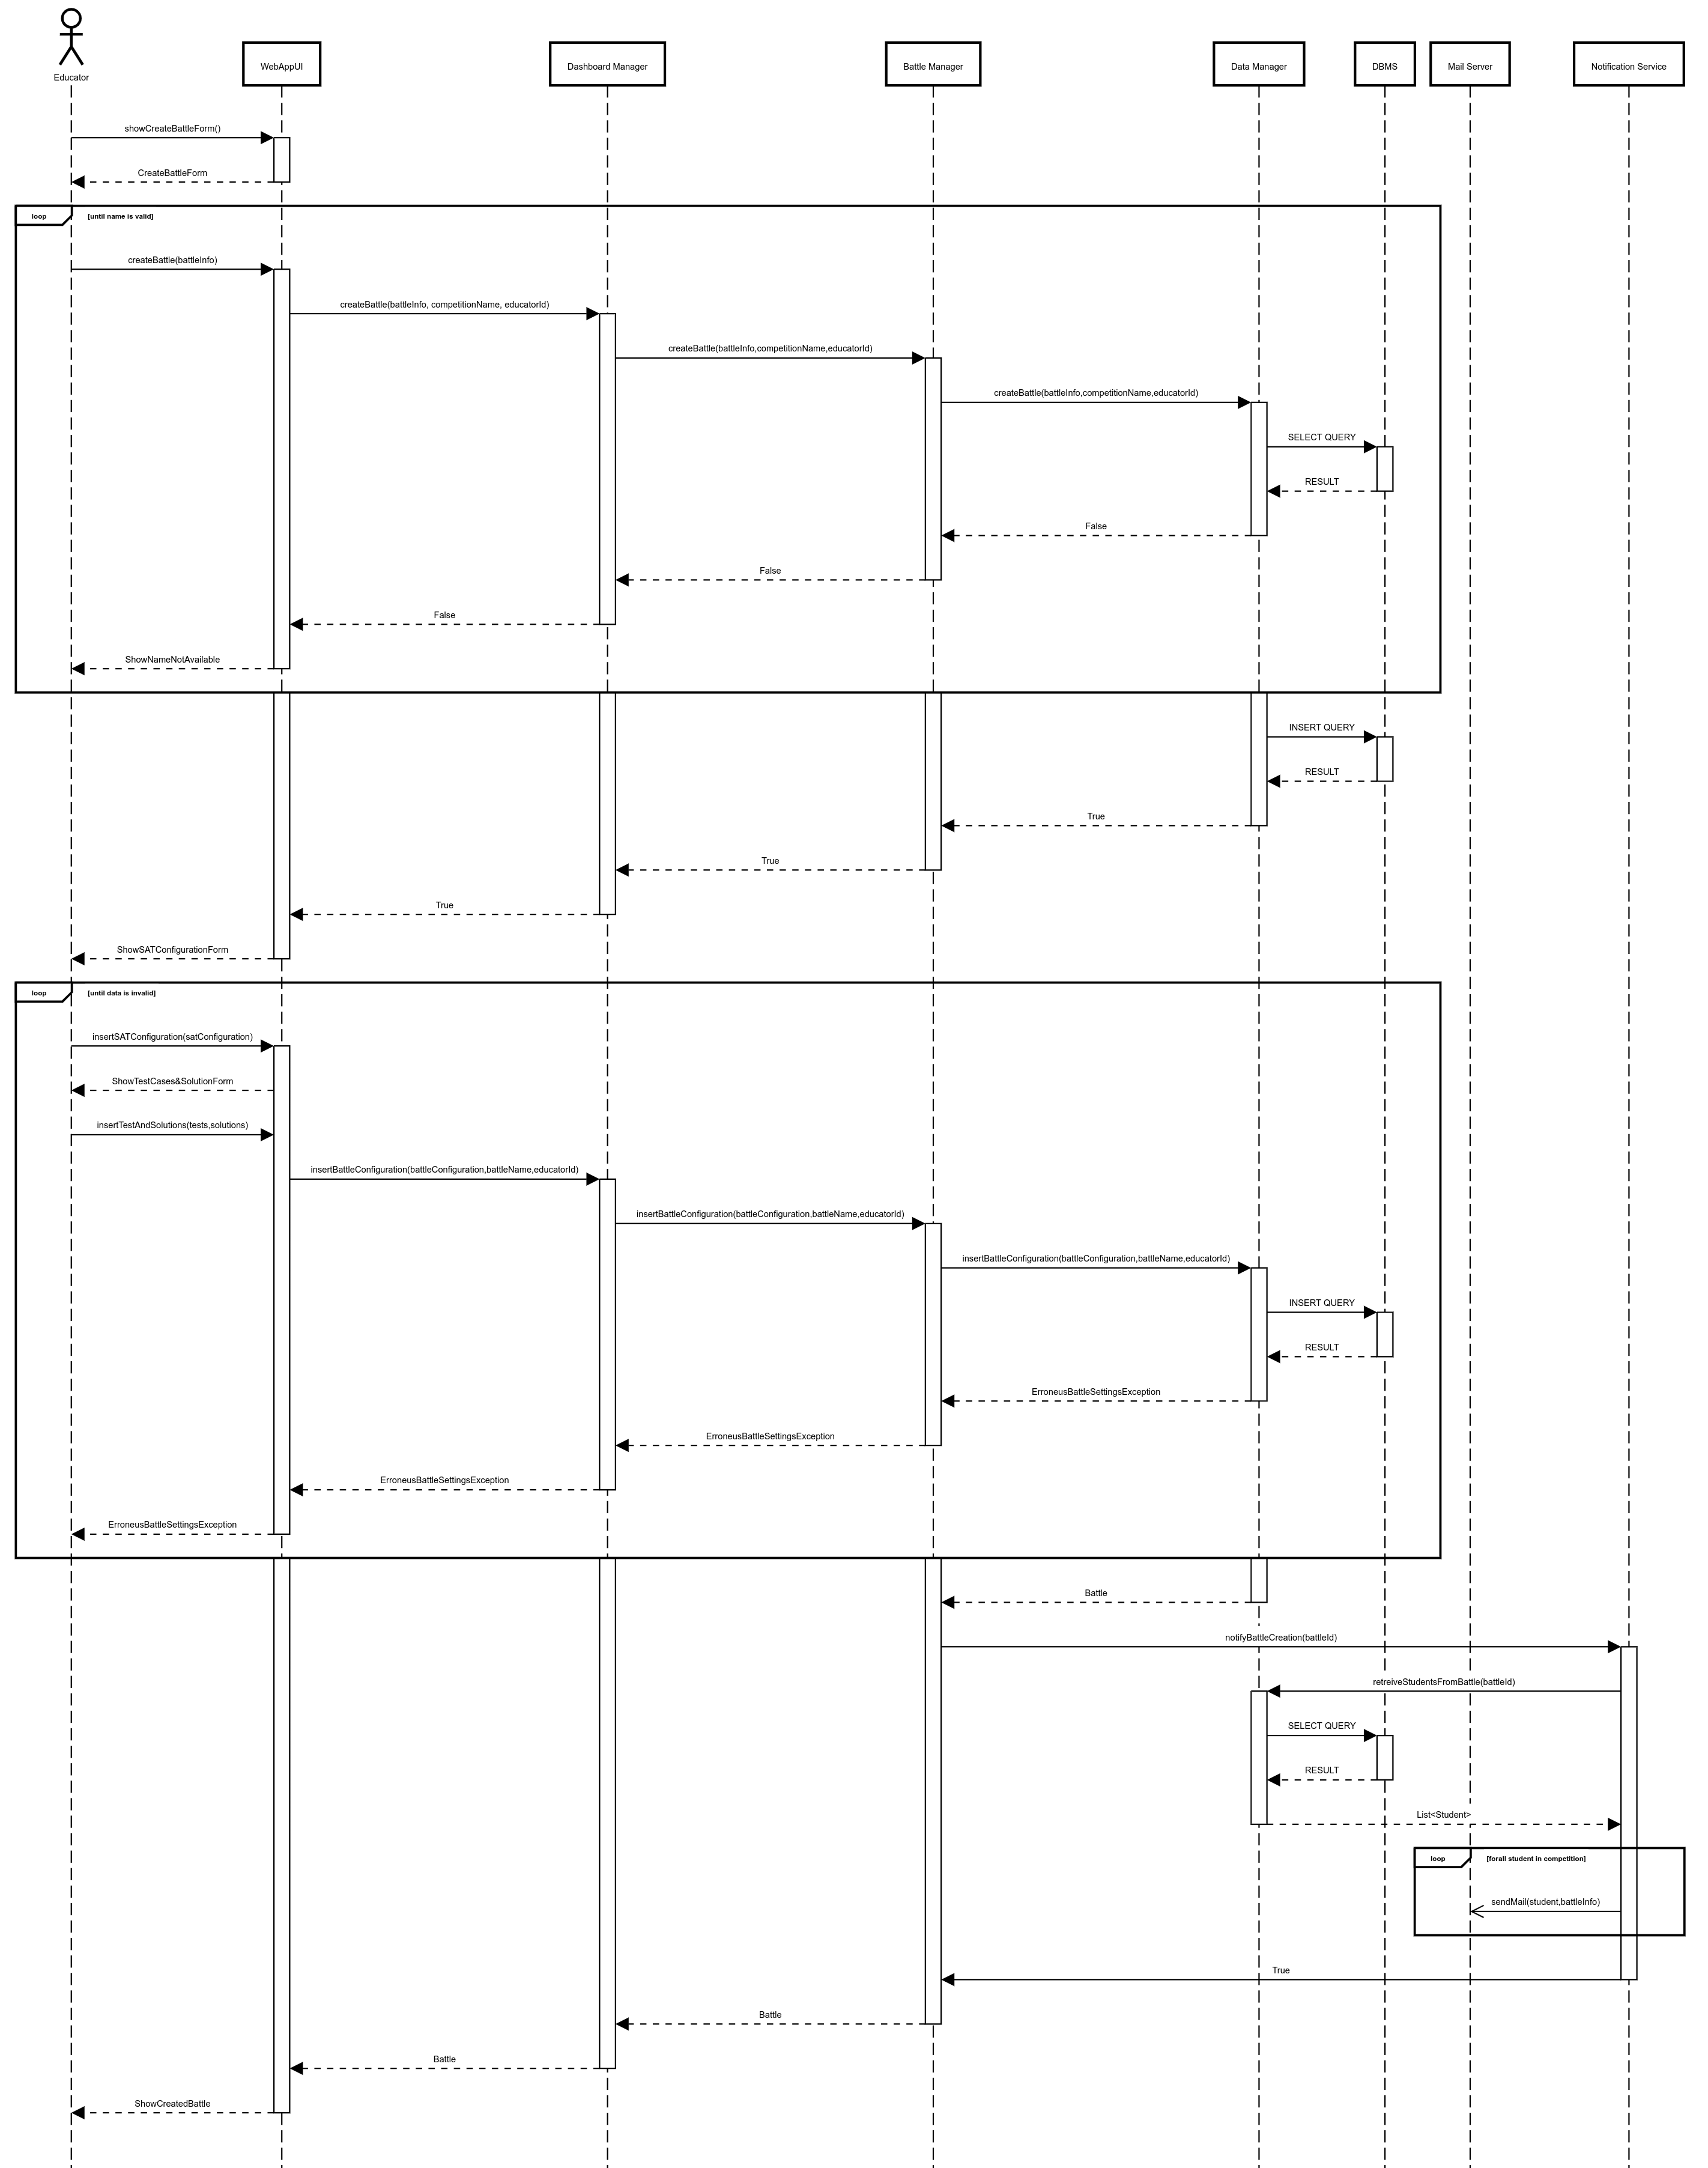
\includegraphics[width=\textwidth,height=0.83\textheight, keepaspectratio]{SequenceDiagrams/06-EducatorCreatesBattle.png}
  \caption{Create battle sequence diagram}
  \label{fig:create_battle_diagramn}
\end{figure}

%9
\subsection*{ST Joins Battle}
To be able to join a battle, a \textit{ST} must be enrolled in a competition and in such competition there has to be at least 1 battle available (subscription deadline not expired). Assuming all those things, when a ST wants to join a battle, he/she has two options: create a team (with the possibility, if enabled by the EDs of the battle, to be a singleton) or to join an already existing team. In the first case the ST has to provide the system all the information needed for the team registration, and if the team has been created correctly he/she can invite other STs to join his/her team (if the ST, owner of the team, wants to participate alone he/she must skip the invite part). In the latter case instead, the ST looks at the list of existing and available teams and if he/she wants to join one of those team they can simply click on the join button.

Since the sequence diagram below was pretty long we decided to split it in two so that it was easier to read it; this means that the two following diagrams are to be understood as consecutive (the [\textit{alt 'ST wants to join an existing public T'}] fragment, in the second part of the diagram, is the [\textit{else}] of the [\textit{alt 'ST selects to create a new T'}] fragment in the first part of the diagram)


\begin{figure}[H]
  \centering
  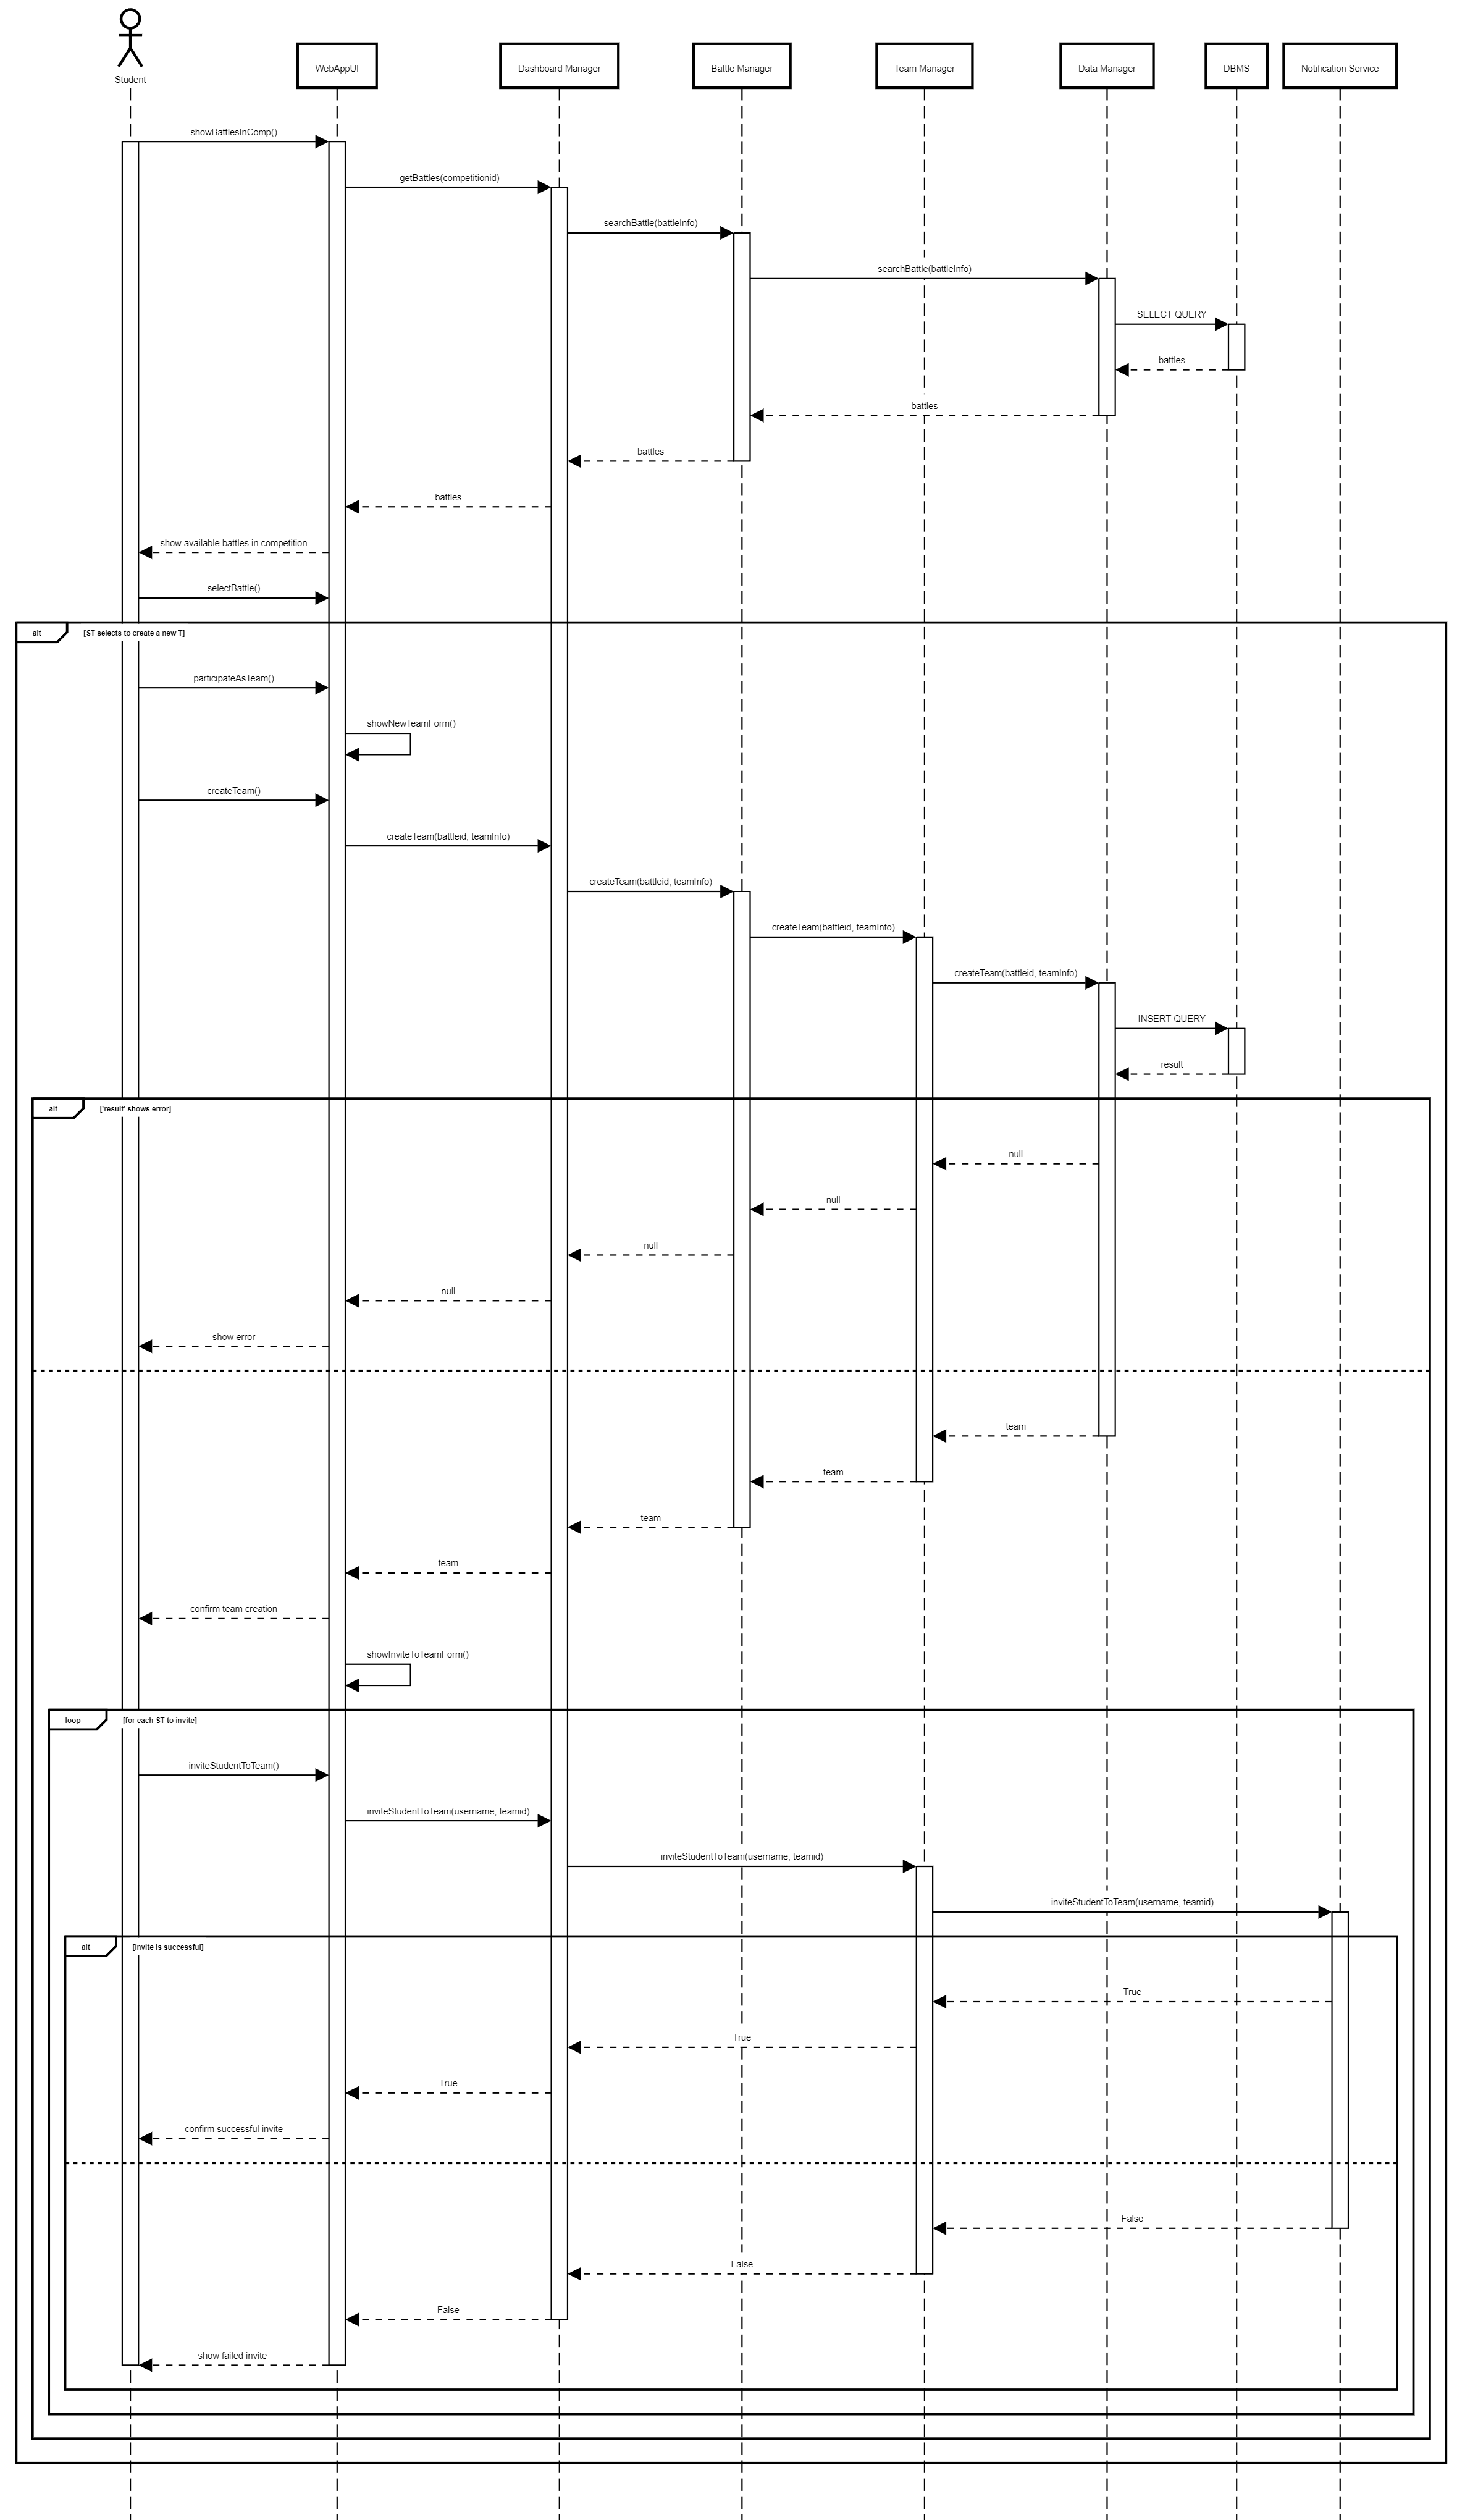
\includegraphics[width=\textwidth,height=\textheight, keepaspectratio]{SequenceDiagrams/09.1-StudentJoinsBattle.png}
  \caption{ST joins battle sequence diagram - Part 1}
  \label{fig:st_joins_battle_1}
\end{figure}

\begin{figure}[H]
  \centering
  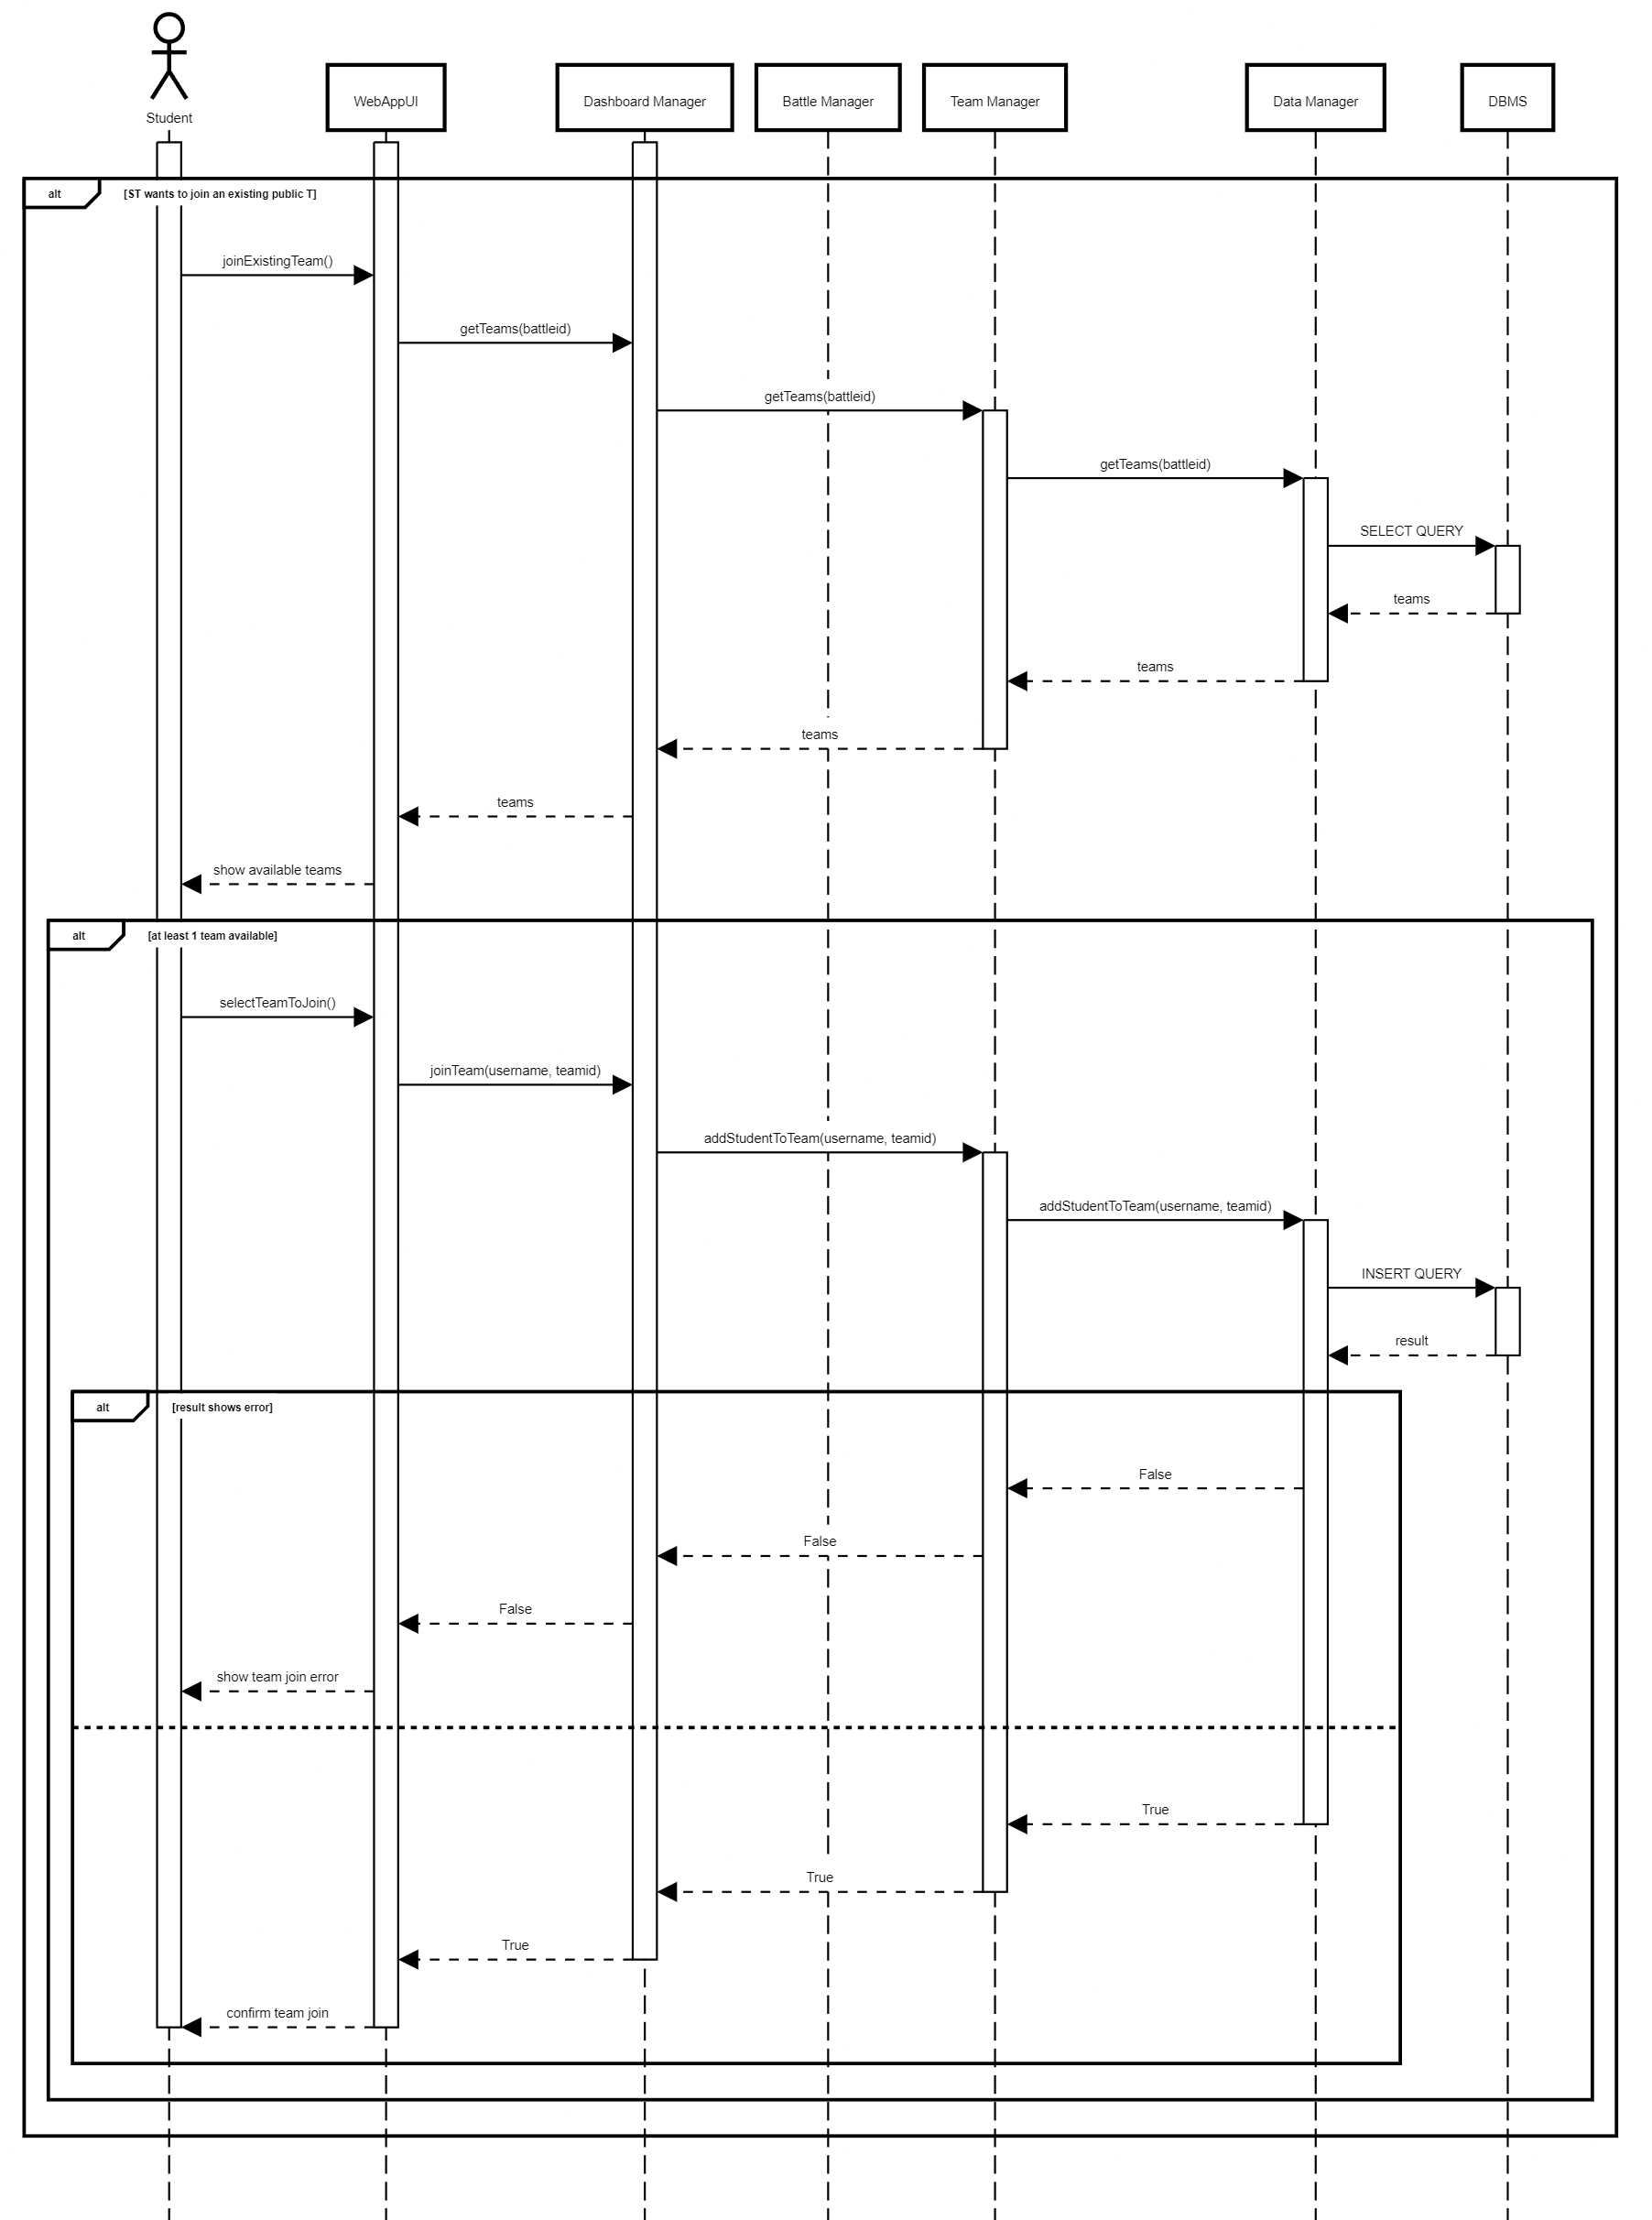
\includegraphics[width=\textwidth, keepaspectratio]{SequenceDiagrams/09.2-StudentJoinsBattle.png}
  \caption{ST joins battle sequence diagram - Part 2}
  \label{fig:st_joins_battle_2}
\end{figure}

%10
\subsection*{User Visualizes battle Rankings}
Assuming that a User (ST or ED) is enrolled firstly in a competition and secondly subscribed to a battle that is still ongoing, such User can see the partial leaderboard of the battle. The sequence diagram below describe exactly this process, starting from the page of the competition. 
\begin{figure}[H]
  \centering
  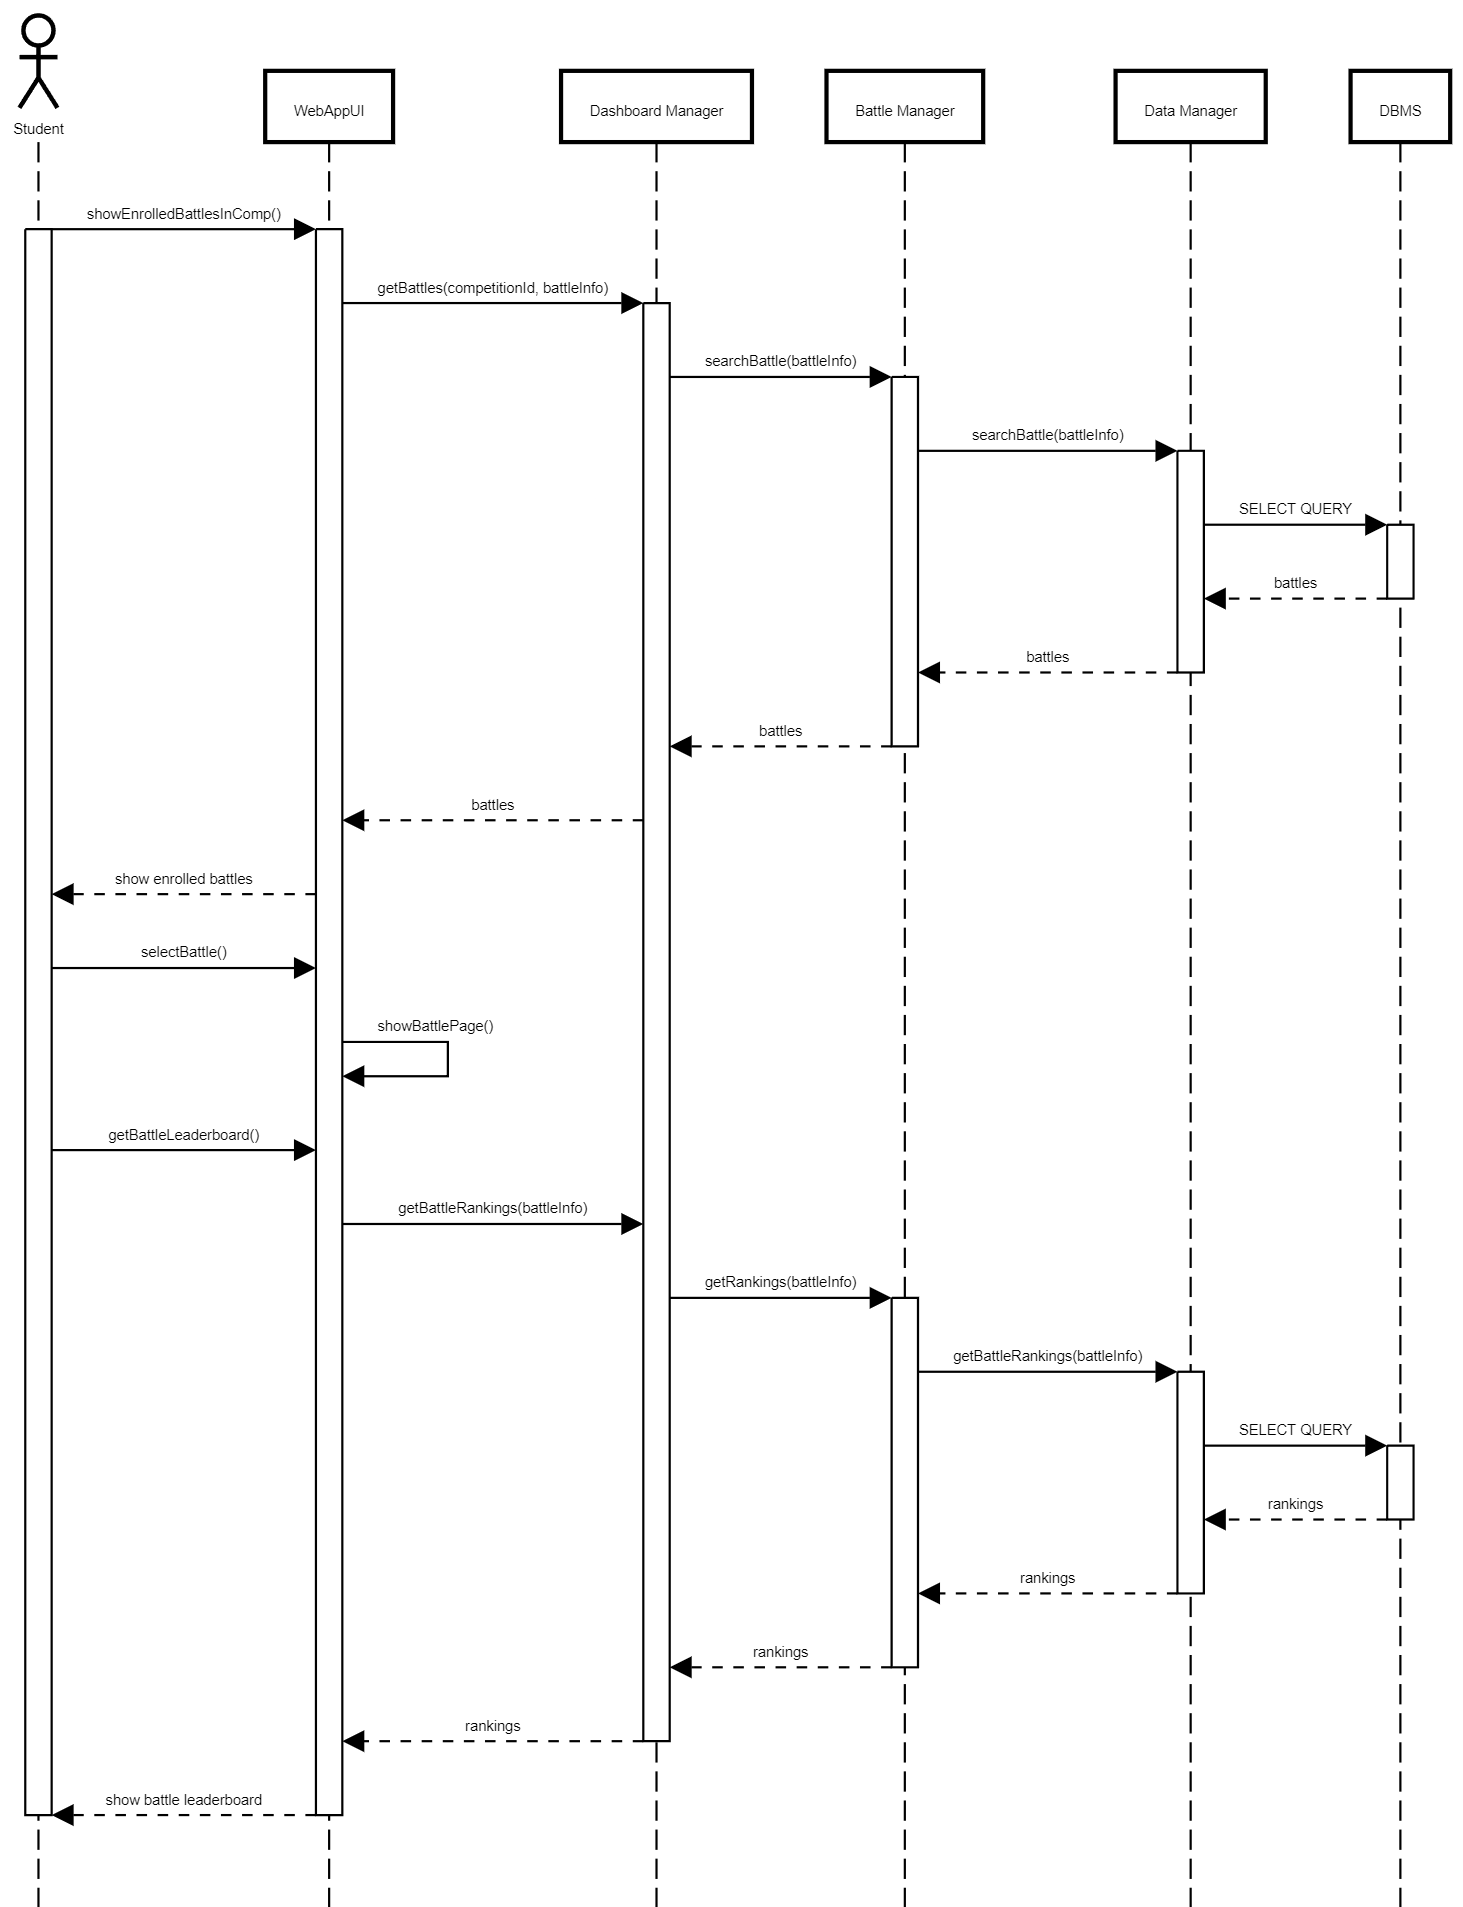
\includegraphics[width=\textwidth,height=0.75\textheight, keepaspectratio]{SequenceDiagrams/10-BattleRankingVisualization.png}
  \caption{Create battle sequence diagram}
  \label{fig:user_visualize_rankings}
\end{figure}

%11
\subsection*{ED Evaluates Code}
An ED can select a T from the list of teams participating to a battle and evaluate its last commit. In particular the ED after selecting the team, he/she can visualize some brief information about the latest commit of the T, from the visualization is possible to navigate to the Github page of the commit. After reviewing the code on Github the ED can return to the CKB page and insert the evaluation of the commit. The process is handled by the \textit{Team Manager} component, which interacts with the \textit{Data Manager} component to insert the evaluation into the DBMS.

\begin{figure}[H]
  \centering
  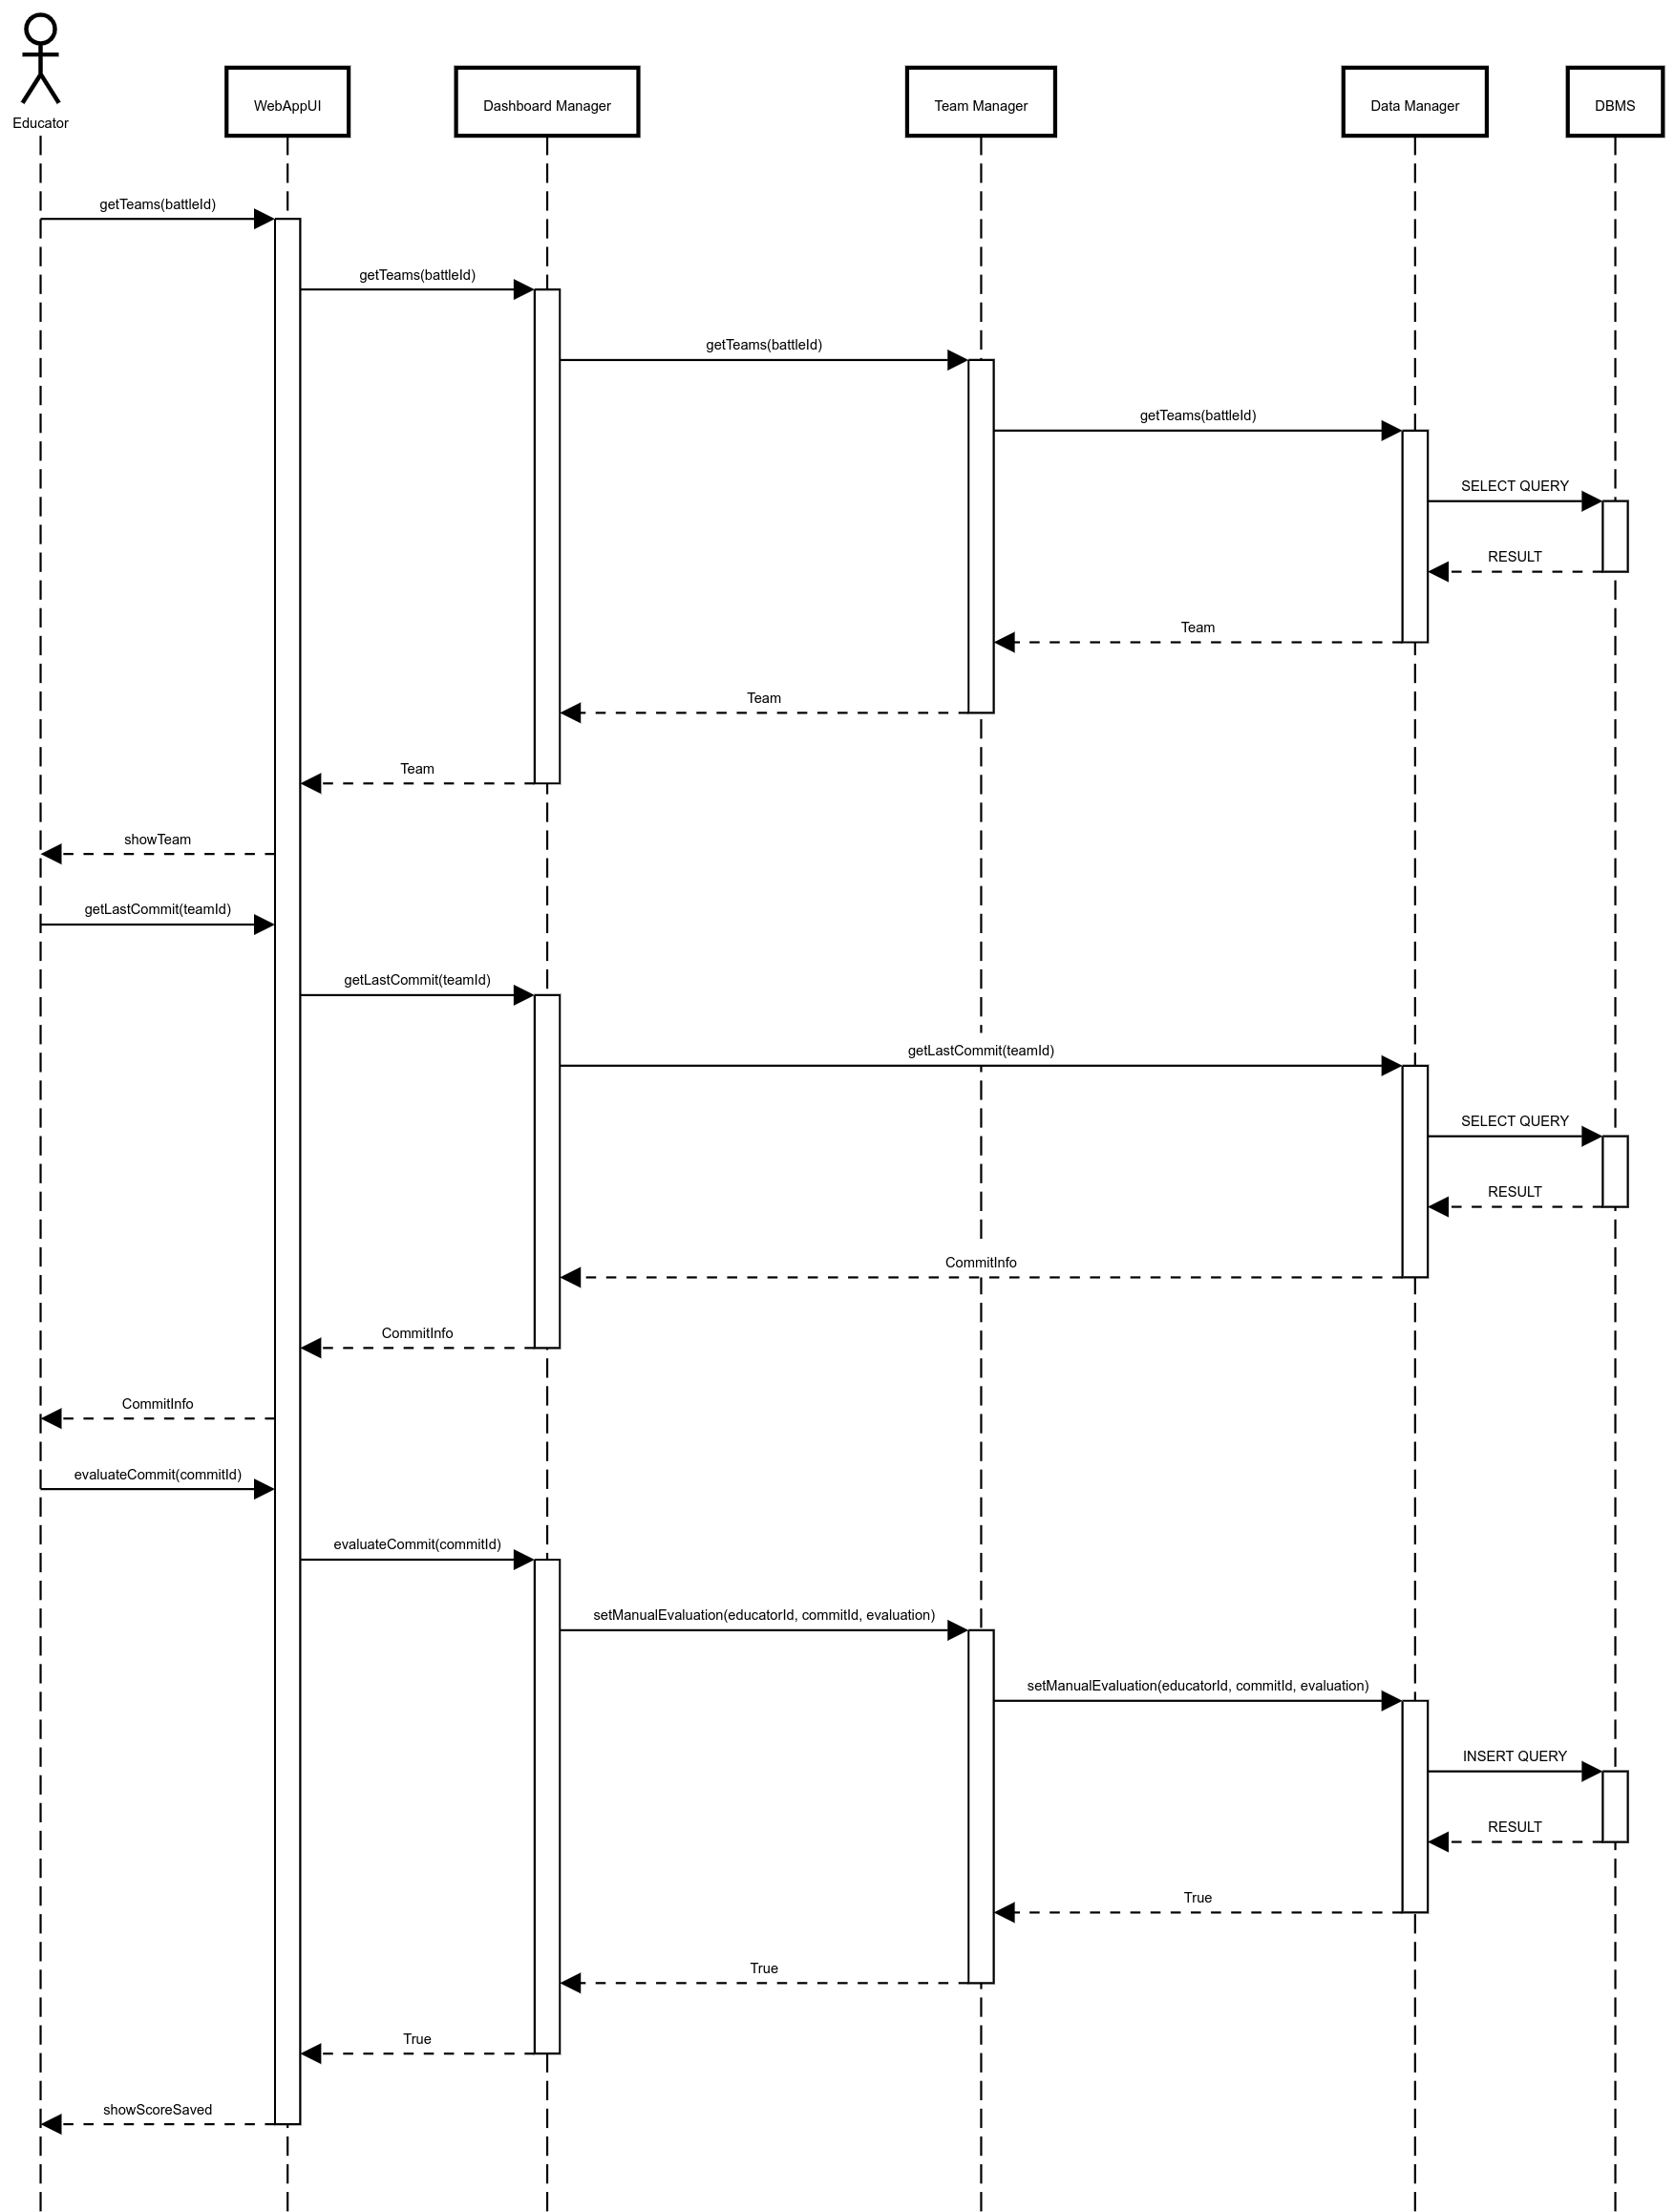
\includegraphics[width=\textwidth,height=0.7\textheight, keepaspectratio]{SequenceDiagrams/11-EdEvaluatesCode.png}
  \caption{ED evaluates code sequence diagram}
  \label{fig:ed_evaluates_code}
\end{figure}

%12
\subsection*{ST Accepts invite}
When a ST clicks on the link in the email received from the system, he/she will be added to the T. The \textit{Team Manager} component will handle the request and will insert the ST into the DBMS using the \textit{Data Manager} component. In case the invitation link is expired, the system will show an error message to the user.

\begin{figure}[H]
  \centering
  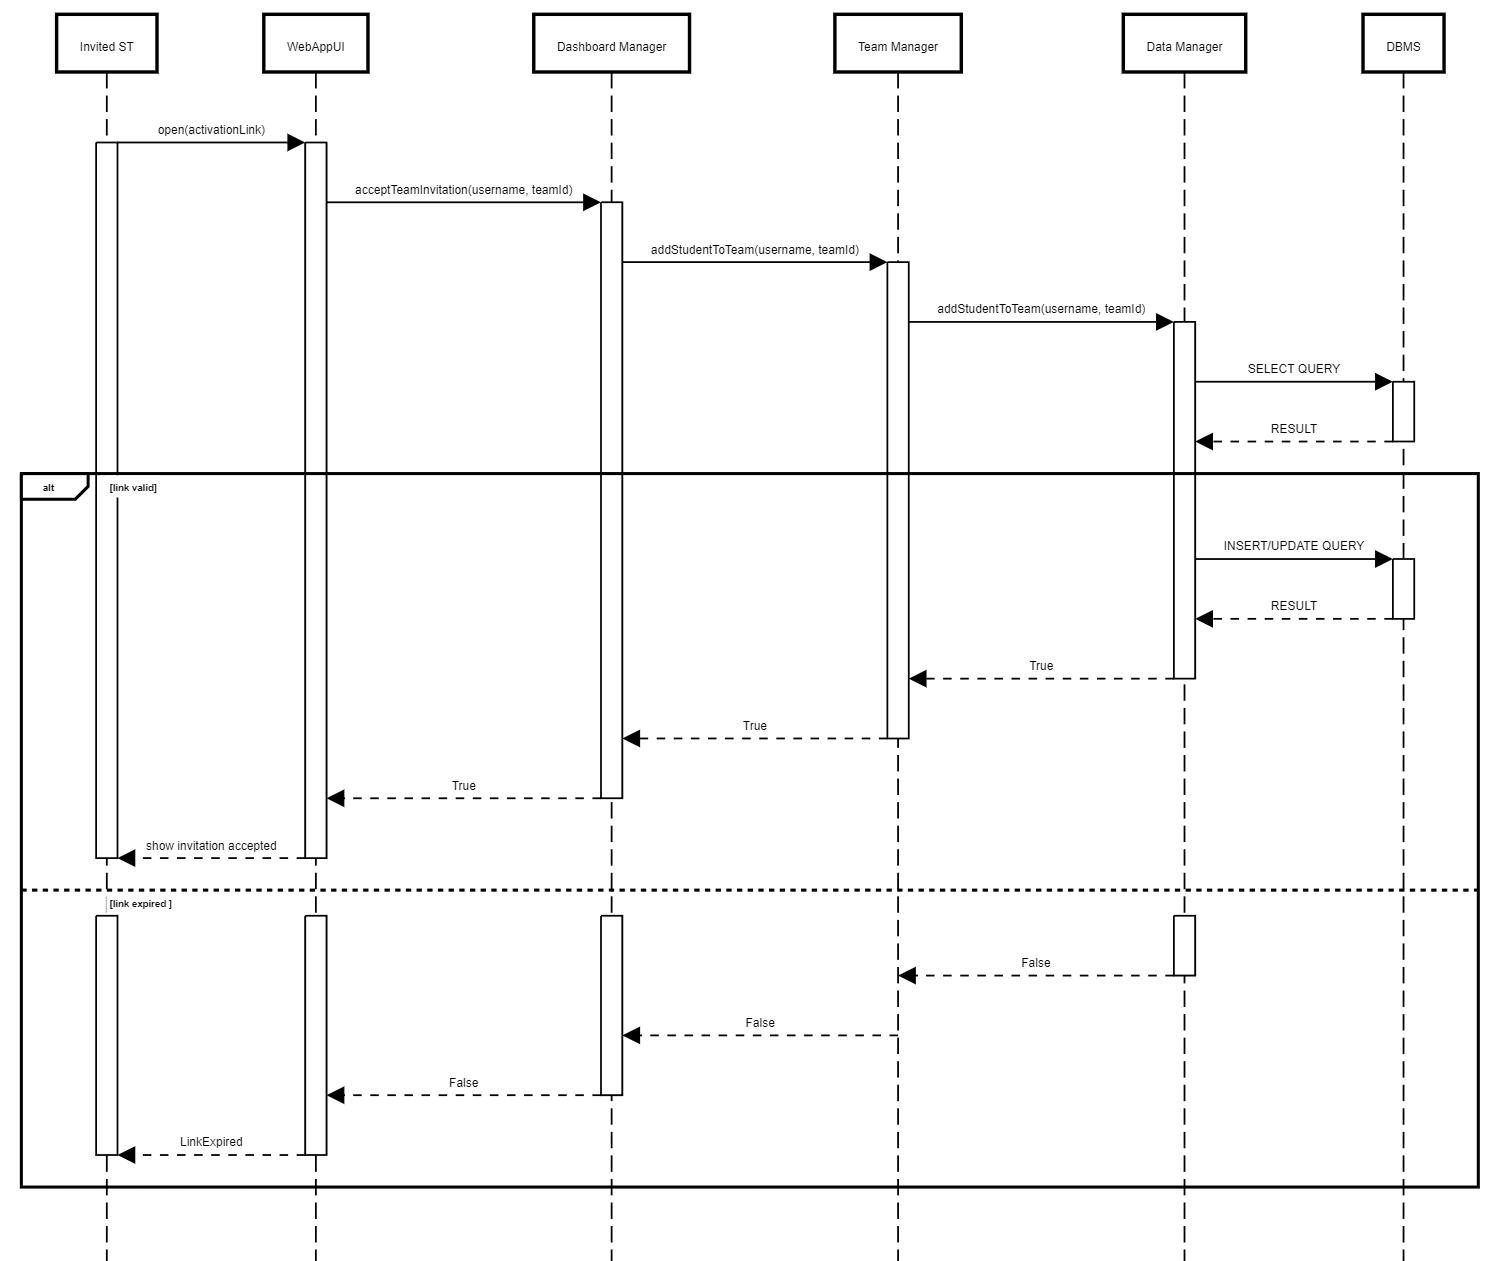
\includegraphics[width=\textwidth,height=\textheight, keepaspectratio]{SequenceDiagrams/12-StAcceptInvite.png}
  \caption{ST accepts invite sequence diagram}
  \label{fig:st_accepts_invite}
\end{figure}

%13
\subsection*{ST Visualizes other ST Profile}
STs can visualize the profile of other STs. The ST can search for a specific ST using its username, the system will show the list of the corresponding STs and the ST can select one of them to visualize its profile. In the profile page the ST can see some information about the ST and the list of the badges that he/she has earned. The \textit{Dashboard Manager} component will handle the request and will retrieve the information from the DBMS using the \textit{Data Manager} component.

\begin{figure}[H]
  \centering
  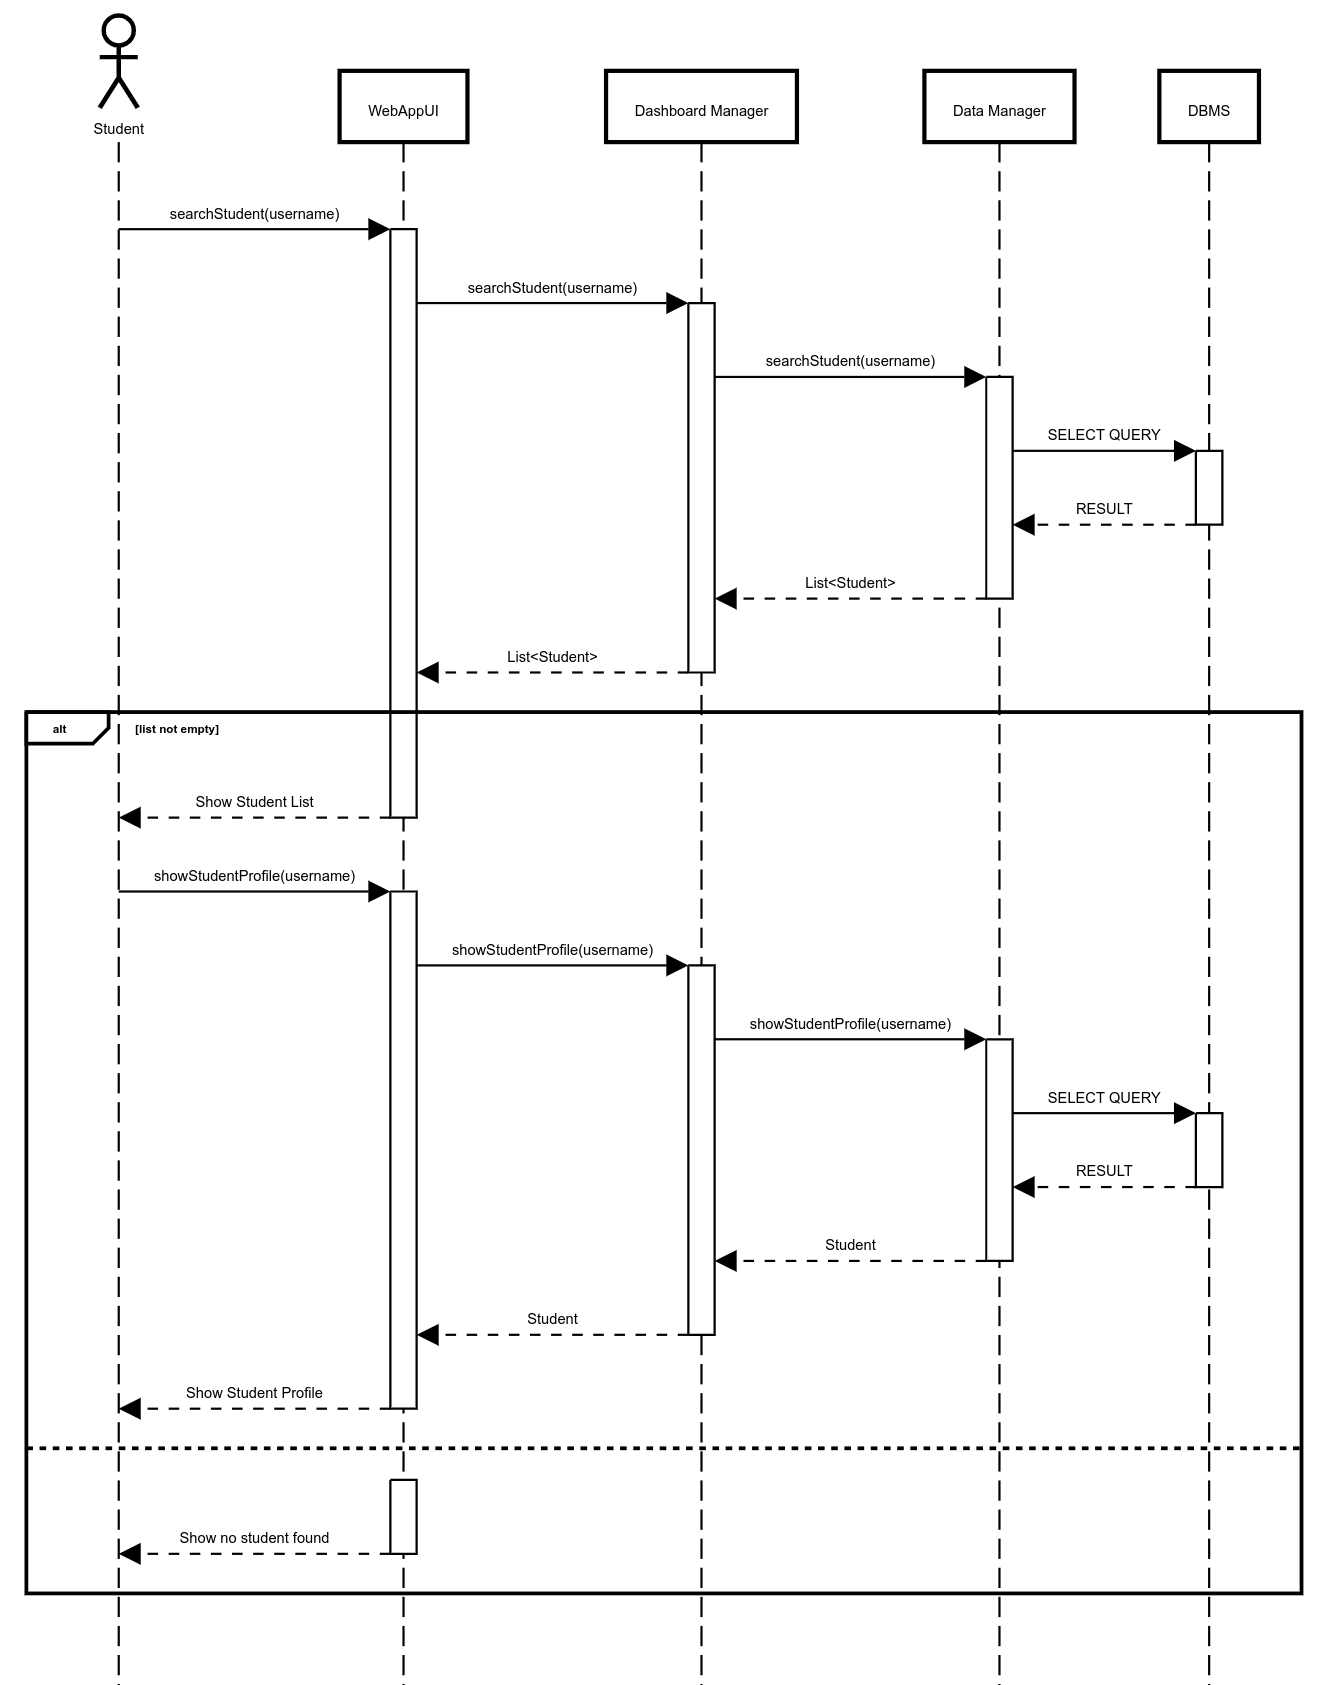
\includegraphics[width=\textwidth,height=\textheight, keepaspectratio]{SequenceDiagrams/13-StudentVisualizeSTprofile.png}
  \caption{ST visualizes other ST profile sequence diagram}
  \label{fig:st_visualizes_other_st_profile}
\end{figure}

\section{Component interfaces}
\label{s:component-interfaces}%


\subsection{Authentication Service}
\subsubsection{AuthInterface}
\begin{itemize}
    \item \texttt{User login(username:String,password:String)}%x
    \item \texttt{bool register(info:UserInfo)} %x
\end{itemize}

\subsection{Data Manager}
\subsubsection{AuthDAOInterface}
\begin{itemize}
    \item \texttt{bool addUser(info: UserInfo)}%x
    \item \texttt{bool checkCredential(username:String,password:String)}%x
    \item \texttt{bool validateNewUser(info:UserInfo)}%x
    \item \texttt{User getUser(username:String)}%x
\end{itemize}

\subsubsection{CompetitionDAOInterface}
\begin{itemize}
    \item \texttt{bool createCompetition(info:CompetitionInfo)}
    \item \texttt{bool addStudentToCompetition(competitionName:String, studentUsername:String)}
    \item \texttt{bool checkEdCanbeInvited(competitionName:String,educatorId:String)}%x
    \item \texttt{Competition getCompetition(name:String)}%x
    \item \texttt{List<Team> getCompRankings(competitionid: String)}
\end{itemize}

\subsubsection{BattleDAOInterface}
\begin{itemize}
    \item \texttt{bool createBattle(competitionName:String, battleInfo:BattleInfo,\\educatorId:String)}%x
    \item \texttt{Set<Battle> searchBattle(battleInfo:BattleInfo)}
    \item \texttt{List<Battle> searchBattleInCompetition(competitionId:String)}%x
    \item \texttt{Battle showBattle(battleName:String)}
    \item \texttt{List<Team> getBattleRankings(battleid: String)}
    \item \texttt{bool insertBattleConfiguration(battleConfiguration:BattleConfiguration,\\battleName:String,educatorId:String)}%x
\end{itemize}

\subsubsection{UserDAOInterface}
\begin{itemize}
    \item \texttt{Team createTeam(battleId:String, teamInfo:TeamInfo)}%x
    \item \texttt{bool removeTeam(teamId:String)}
    \item \texttt{bool addStudentToTeam(username:String,teamId:String)}%x
    \item \texttt{bool setManualEvaluation(educatorId:String,commitId:String,evaluation: Evaluation)}%x
    \item \texttt{Team getTeams(battleid: String)}%x
\end{itemize}

\subsubsection{BadgeDAOInterface}
\begin{itemize}
    \item \texttt{Set<User> retrieveUsersFromCompetition(competitionName:String)}
    \item \texttt{BadgeRule getBadgeRule(badge: Badge)}
    \item \texttt{bool removeBadge(badge:Badge)}
    \item \texttt{bool assignBadge(username:String, badge:Badge)}
    \item \texttt{bool createBadge(educatorId:String,competitionId:String, badgeInfo:BadgeInfo)}%x
\end{itemize}

\subsubsection{NotificationDAOInterface}
\begin{itemize}
    \item \texttt{Set<Student> retrieveStudentsFromTeam(teamId:String)}
    \item \texttt{Set<User> retrieveUsersFromCompetition(competitionId:String)}
    \item \texttt{Set<Student> retrieveStudentsFromCompetition(competitionId:String)}%x
    \item \texttt{Set<Educator> retrieveEducatorsFromCompetition(competitionId:String)}
    \item \texttt{Set<User> retrieveUsersFromBattle(battleId:String)}
    \item \texttt{Set<Student> retrieveStudentsFromBattle(battleId:String)}
    \item \texttt{Set<Educator> retrieveEducatorsFromBattle(battleId:String)}
    \item \texttt{Educator retrieveEducatorInfo(educatorId:String)}%x
\end{itemize}

\subsubsection{PointsAPI}
\begin{itemize}
    \item \texttt{bool addEvaluationToTeam(teamId:string, evaluation:Evaluation)}
\end{itemize}

\subsubsection{DashboardDAOInterface}
\begin{itemize}
    \item \texttt{List<Student> searchStudent(studentName:String)}%x
    \item \texttt{Student showStudentProfile(username:String)}%x
    \item \texttt{CommitInfo getLastCommit(teamId: String)}%x
\end{itemize}

\subsection{Dashboard Manager}
\subsubsection{DashboardInterface}
\begin{itemize}
    \item \texttt{DashboardInfo getDashboardInfo(User)}%x
    \item \texttt{createCompetition(competitionInfo:CompetitionInfo)}%x
    \item \texttt{bool createBattle(battleInfo:BattleInfo,competitionName:String,\\educatorId:String)}%x
    \item \texttt{bool joinCompetition(competitionName:String, studentUsername:String)}%x
    \item \texttt{CompetitionInfo showCompetition(name:String)}%x
    \item \texttt{List<Battle> getBattles(competitionid: String)}%x
    %@toCheck
    \item \texttt{Battle getBattle(competitionid: String, battleId: String)}
    %\item \texttt{bool insertSATConfiguration(satConfiguration:SatConfiguration,\\battleName:String,educatorId:String)}%x
    \item \texttt{bool insertBattleConfiguration(battleConfiguration:BattleConfiguration, \\battleName:String,educatorId:String)}%x
    \item \texttt{bool inviteStudentToTeam(username: String, teamid: String)}%x
    \item \texttt{List<Team> getTeams(battleid: String)}%x
    \item \texttt{bool joinTeam(username: String,teamid: String)}%x
    \item \texttt{List<Team> getCompRankings(competitionid: String)}
    \item \texttt{List<Team> getBattleRankings(battleInfo: BattleInfo)}
    \item \texttt{List<Student> searchStudent(studentName:String)}%x
    \item \texttt{Student showStudentProfile(username:String)}%x
    \item \texttt{CompetitionSetting showCompetitionSettings(educatorId:String,\\competitionId:String)}%x
    \item \texttt{BadgeCreation showBadgeCreation(educatorId:String,\\competitionId:String)}%x
    \item \texttt{InviteEdPanel showInviteEd(educatorId:String,competitionId:String)}%x
    \item \texttt{bool inviteED(educatorId:String,competitionId:String,invitedEducatorId:String)}%x
    \item \texttt{bool createBadge(educatorId:String,competitionName:String, badgeInfo: BadgeInfo)}%x
    \item \texttt{CommitInfo getLastCommit(teamId: String)}%x
    \item \texttt{bool acceptInvitation(educatorId:String,competitionId:String)}%x
    \item \texttt{bool acceptTeamInvitation(username:String,teamId:String)}%x
    \item \texttt{Team createTeam(battleid: String, username: String)}%x
    \item \texttt{bool evaluateCommit(commitId: String)}%x
\end{itemize}

\subsection{Competition Manager}
\subsubsection{CompetitionInterface}
\begin{itemize}
    \item \texttt{Competition createCompetition(info:CompetitionInfo)}%x
    \item \texttt{Set<Competition> searchCompetition(info:CompetitionInfo)}
    \item \texttt{bool deleteCompetition(name:String)}
    \item \texttt{Competition getCompetition(name:String)}%x
    \item \texttt{bool addManager(competitionName:String,username:String)}%x
    \item \texttt{bool removeManager(competitionName:String,username:String)}
    \item \texttt{bool endCompetition(competitionName:String)}
    \item \texttt{bool joinCompetition(competitionName:String, studentUsername:String)}%x
    \item \texttt{bool createBadge(educatorId:String,competitionName:String, badgeInfo: BadgeInfo)}%x
    \item \texttt{bool removeBadge(badgeId:String)}
    \item \texttt{List<Team> getRankings(competitionid: String)}
    \item \texttt{bool acceptInvitation(educatorId:String,competitionId:String)}%x
    \item \texttt{bool inviteED(educatorId:String,competitionId:String,invitedEducatorId:String)}%x
\end{itemize}

\subsection{Badge Manager}
\subsubsection{BadgeInterface}
\begin{itemize}
    \item \texttt{bool createBadge(competitionName:String, badgeInfo: BadgeInfo)}%x
    \item \texttt{bool assignBadges(competitionName:String)}
    \item \texttt{bool removeBadge(badgeId:String)}
\end{itemize}

\subsection{BattleManager}
\subsubsection{BattleInterface}
\begin{itemize}
    \item \texttt{bool createBattle(competitionName:String, battleInfo:BattleInfo,\\ educatorId:String)}
    \item \texttt{Team createTeam(battleId:String, teamInfo:TeamInfo)}%x
    \item \texttt{bool removeTeam(teamId:String)}
    \item \texttt{List<Battle> searchBattle(battleInfo:BattleInfo)}
    \item \texttt{List<Battle> searchBattleInCompetition(competitionId:String)}%x
    \item \texttt{Battle showBattle(battleName:String)}
    \item \texttt{bool deleteBattle(battleName:String)}
    %\item \texttt{insertSATConfiguration(satConfiguration,battleName,educatorId)}
    \item \texttt{bool insertBattleConfiguration(battleConfiguration:BattleConfiguration, \\battleName:String,educatorId:String)}%x
    \item \texttt{List<Team> getRankings(battleid: String)}
\end{itemize}

\subsection{Team Manager}
\subsubsection{TeamHandlerInterface}
\begin{itemize}
    \item \texttt{Team createTeam(battleId:String, teamInfo:TeamInfo)}
    \item \texttt{bool removeTeam(teamId:String)}
    \item \texttt{Team getTeams(battleid: String)}%x
\end{itemize}

\subsubsection{TeamInterface}
\begin{itemize}
    \item \texttt{bool addStudentToTeam(username:String,teamId:String)}%x
    \item \texttt{bool inviteStudentToTeam(username:String,teamId:String)}%x
    \item \texttt{bool setManualEvaluation(educatorId:String,commitId:String,evaluation: Evaluation)}%x
\end{itemize}


\subsection{Notification Service}
\subsubsection{InviteInterface}
\begin{itemize}
    \item \texttt{bool inviteStudentToTeam(username:String,teamId:String)}%x
\end{itemize}

\subsubsection{NotifyBattleInterface}
\begin{itemize}
    \item \texttt{bool notifyBattleCreation(battleId:String, competitionId:String)}%x
    \item \texttt{bool notifyStartedBattle(battleId:String,username:String)}
    \item \texttt{bool notifyEndBattle(battleId:String,username:String)}
    \item \texttt{bool notifyManageBattle(battleId:String,username:String)}
\end{itemize}

\subsubsection{NotifyCompInterface}
\begin{itemize}
    \item \texttt{bool notifyNewCompetion(competitionId:String,username:String)}
    \item \texttt{bool notifyNewBattle(competitionId:String, battleId:String,username:String)}
    \item \texttt{bool notifyEdInvitation(competitionId:String,invitedEd:String)}%x
    \item \texttt{bool notifyManageCompetition(competitionId:String,username:String)}
\end{itemize}

\subsubsection{NotifyAuthInterface}
\begin{itemize}
    \item \texttt{bool NotifyUserRegistration(User)}%x
\end{itemize}

\subsection{Evaluator Controller}
\subsubsection{EvaluationAPI}
\begin{itemize}
    \item \texttt{bool pullCode(authorId:String, commitId:String)}
\end{itemize}

\subsection{Code Evaluator}
\subsubsection{EvaluatorInterface}
\begin{itemize}
    \item \texttt{bool evaluateCode(authorId:String, commitId:String)}
    \item \texttt{void setConf(conf: EvalConfig)}
\end{itemize}

\subsection{Static Analyzer}
\subsubsection{AnalyzerInterface}
\begin{itemize}
    \item \texttt{bool evaluateCode(authorId:String, commitId:String, params:String)}
    \item \texttt{void setConf(conf: StatConfig)}
\end{itemize}

\subsection{Point Manager}
\subsubsection{EvaluationPointsInterface}
\begin{itemize}
    \item \texttt{bool assignPoint(authorId:String, evalResults: EvalResults)}
\end{itemize}

\subsubsection{StaticPointsInterface}
\begin{itemize}
    \item \texttt{bool assignPoint(authorId:String, statResults: StatResults)}
\end{itemize}

\subsubsection{ScoreInterface}
\begin{itemize}
    \item \texttt{void setEvalScoreFunction(conf: EvalScoreFunction)}
    \item \texttt{void setStatAnalysisScoreFunction(conf: StatScoreFunction)}
\end{itemize}

\newpage

\section{Selected architectural styles and patterns}
\label{s:selected-architectural-styles-and-patterns}%

\subsection{Client-Server}
Since the CKB is a platform offered through the web, the client-server architecture is the most suitable for this kind of application. In particular we are using a 3-tier architecture, where the client is the web browser, the server is the application server and the database is the data server. This architecture is the most suitable for our application because it allows us to separate the presentation layer from the business logic and the data layer. Moreover, this separation allows us to have a more maintainable and scalable application.

\subsection{REST}
The communication between the client and the server is based on the REST architectural style. The REST architectural style is stateless, this means that the server does not need to store any information about the client session, this allows us to have a more scalable application. Moreover, in combination with the HTTP protocol, it allows us to provide a uniform interface to the client, which is based on the HTTP methods (GET, POST, PUT, DELETE).

\subsection{MVC}
The MVC pattern is used to separate the presentation layer from the business logic. In particular, the \textit{Model} contains the definition of all the elements of our application, the \textit{View} is represented by the \textit{WebAppUI} component and the \textit{Controller} is represented by all the other \textit{Managers} component. This pattern allows us to have a more maintainable application, because the changes in one layer do not affect the other layers.


\section{Other design decisions}
\label{s:other-design-decisions}%

\subsection{SandBox}
\label{ss:other-design-decisions-sandbox}%
To protect the application from malicious code, we decided to use a sandbox. In particular, the code evaluator and the static analyzer will be executed in a sandbox. This allows us to have a more secure application, because the code will be executed in a controlled environment.


\subsection{Database}
\label{ss:other-design-decisions-database}%
We decided to use a relational database to store the data of the application given its structure. In particular, we decided to use PostgreSQL, because it is an open source database and it is one of the most used relational database. Moreover, it is ACID compliant, this means that it guarantees the atomicity, consistency, isolation and durability of the transactions.
